\documentclass[aspectratio=169, usenames, dvipsnames]{beamer}

%%%%%
%%%%%
%%%%%     DEFINE THE THEME USED
%%%%%
%%%%%

\usetheme{jc}

%%%%%
%%%%%
%%%%%     LIST OF PACKAGES USED
%%%%%
%%%%%

\graphicspath{{imgs/}}

\usepackage[utf8]{inputenc}
\usepackage[T1]{fontenc}

\usepackage[]{nicefrac}

\usepackage[]{amsmath, amssymb, amsfonts}
\usepackage[]{bm}

\usepackage[]{graphicx}

\usepackage{xcolor}
\usepackage{tikz}
\usetikzlibrary{decorations.pathreplacing}
\usetikzlibrary{backgrounds, matrix}
\usetikzlibrary{arrows, shapes}
\usetikzlibrary{tikzmark}
\usetikzlibrary{calc}
\usetikzlibrary{positioning}
\usetikzlibrary{shadows}
\usetikzlibrary{trees, mindmap}

\usepackage{pgfplots}
\pgfplotsset{compat=newest}


\newcommand{\highlight}[2]{\colorbox{#1!17}{$\displaystyle #2$}}
\newcommand{\highlightdark}[2]{\colorbox{#1!47}{$\displaystyle #2$}}
\renewcommand{\highlight}[2]{\colorbox{#1!17}{#2}}
\renewcommand{\highlightdark}[2]{\colorbox{#1!47}{#2}}


\DeclareMathOperator*{\minimize}{minimize~}
\DeclareMathOperator*{\maximize}{maximize~}
\DeclareMathOperator*{\subto}{subject~to~}

%%%%%
%%%%%
%%%%%     INFO ABOUT THE PRESENTATION
%%%%%
%%%%%

\title{On the importance of low-dimensional structures for data-driven modeling}
\author[JC]{Jean-Christophe Loiseau}
\date[]{May, 13\textsuperscript{th} 2022}

%%%%%
%%%%%
%%%%%     PRESENTATION
%%%%%
%%%%%

\begin{document}

\begin{frame}
  \titlepage
\end{frame}

%% \begin{frame}[t, c]{blabla}
%%   \vfill

%%   \centering

%%   This is a test

%%   \vfill

%%   \begin{tcolorbox}[enhanced, coltitle=black, coltext=white, colback=black, title=My title, frame style tile={width=\paperwidth}{background.jpg}]
%%     Hello
%% \end{tcolorbox}

%%   \vfill
%% \end{frame}

\begin{frame}
  \vfill
  \begin{minipage}{.68\textwidth}
    \begin{itemize}
    \item Maître de Conférences in Fluid Dynamics and Applied Math.

      \bigskip

    \item Machine-learning enthusiast with application to engineering systems.

      \bigskip

    \item Data-efficient models with guarantees of optimality or interpretability.
    \end{itemize}
  \end{minipage}%
  \hfill
  \begin{minipage}{.28\textwidth}
    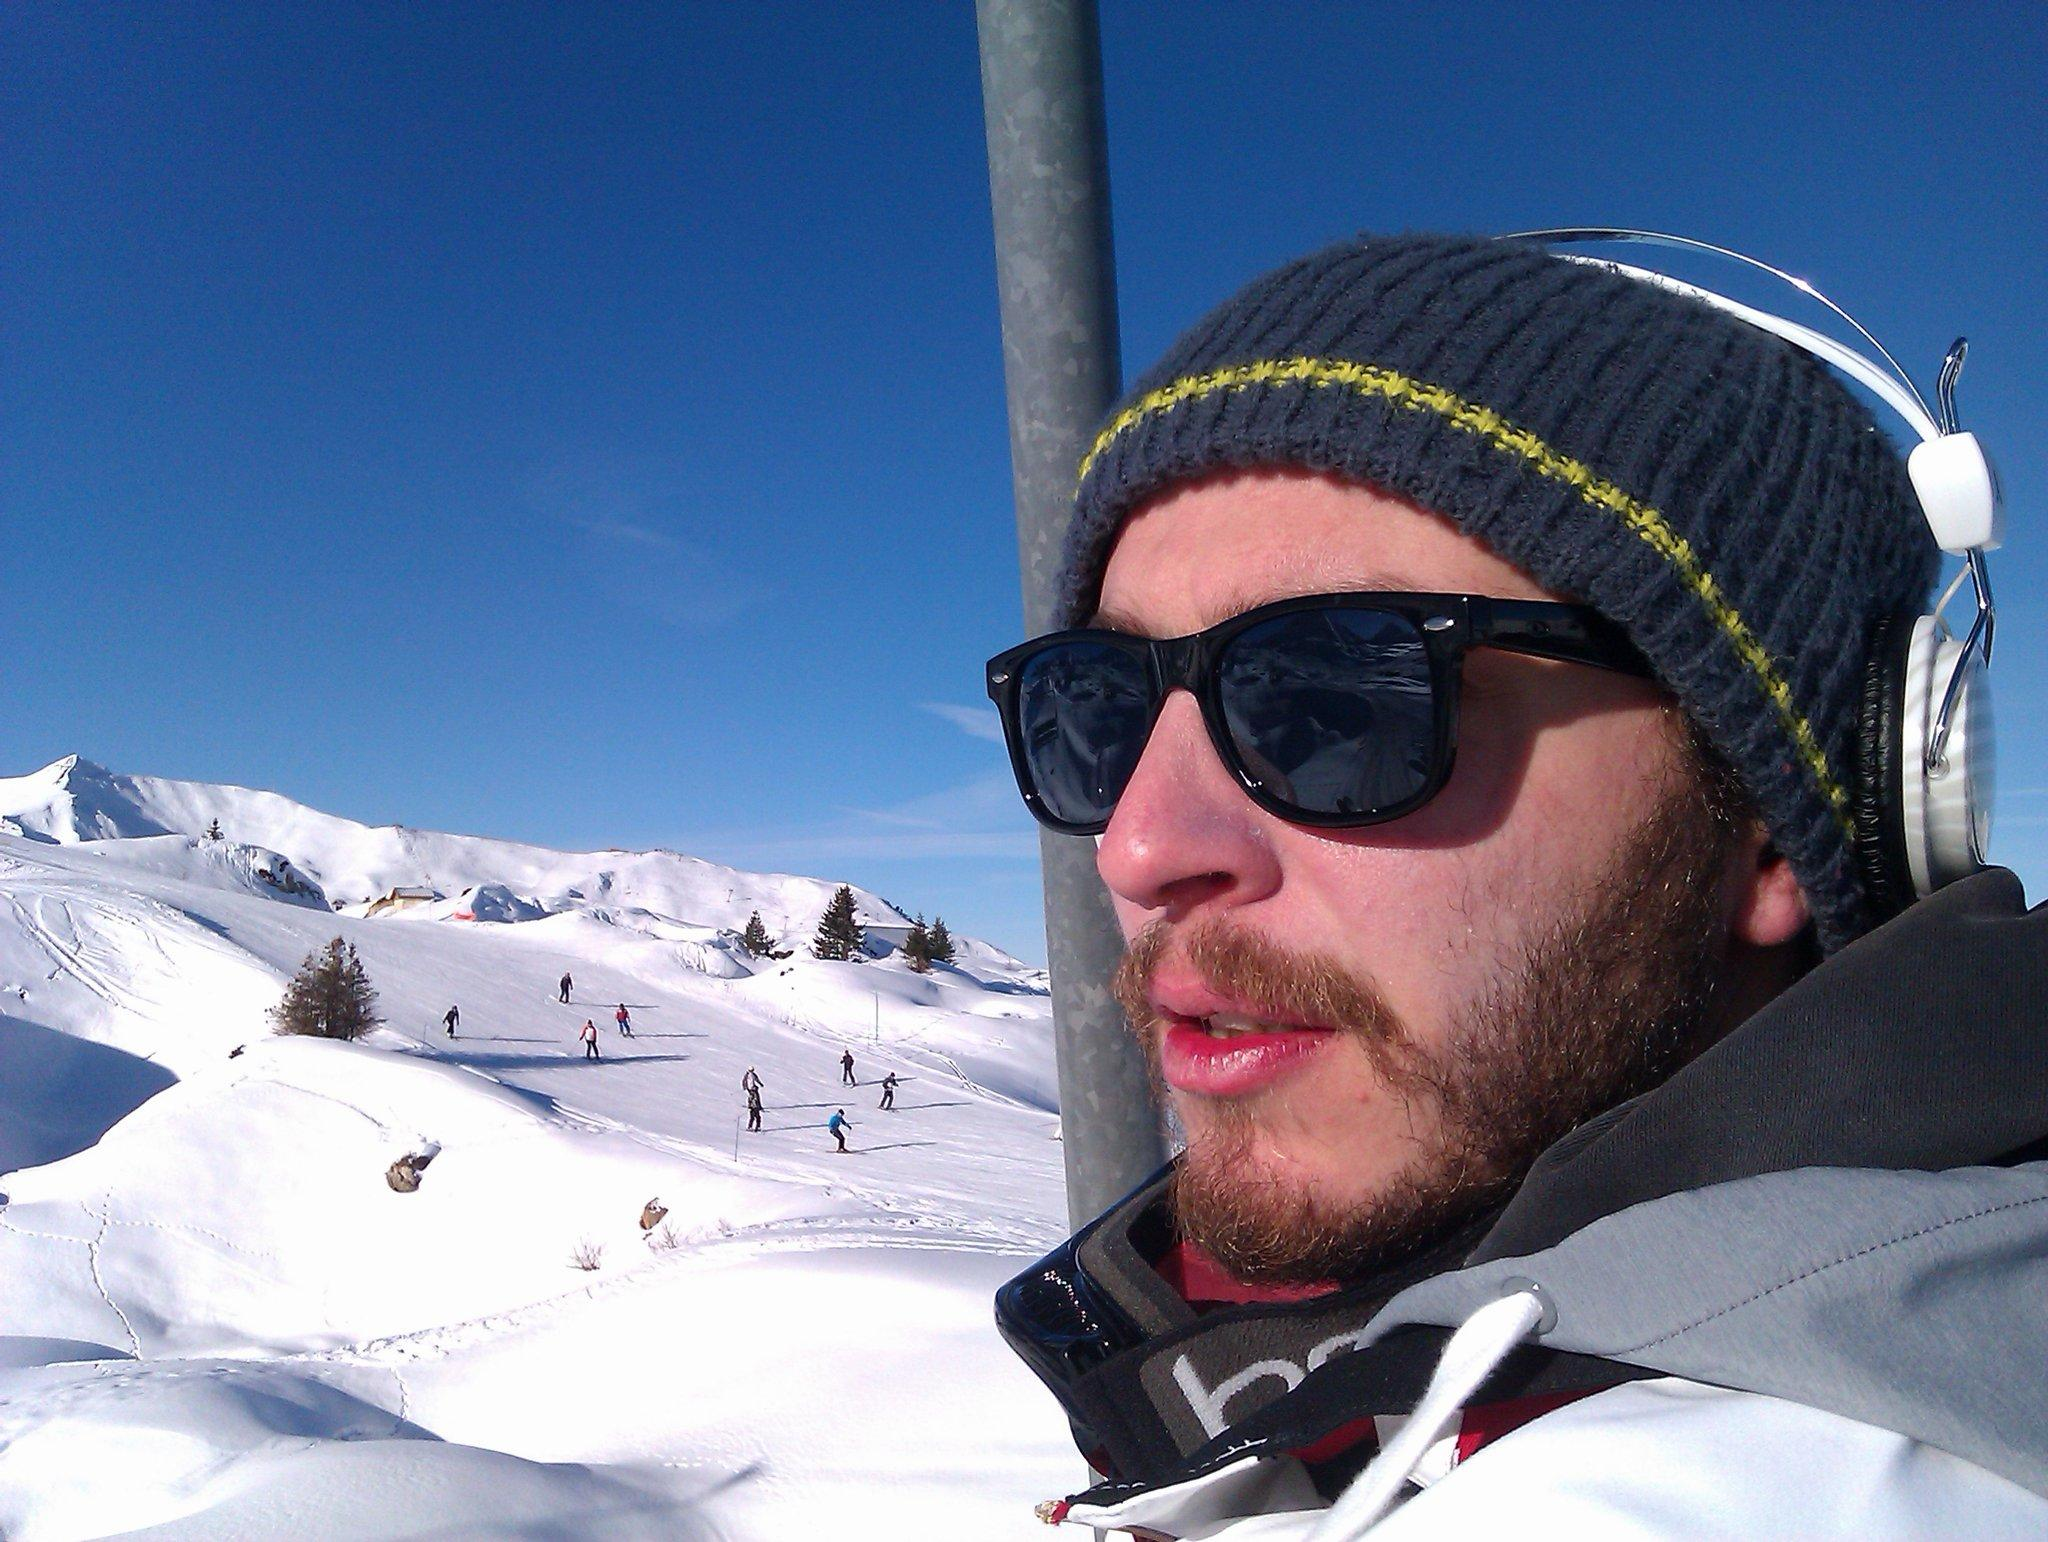
\includegraphics[width=\textwidth]{myself}
  \end{minipage}

  \vfill
\end{frame}

\section{A brief overview of SVD}
\begin{frame}
  \sectionpage
\end{frame}

\begin{frame}
  \vfill

  \begin{overprint}

    \onslide<1>
    \Large
    \[
    \bm{A} = {\highlightdark{black!100}{$\bm{U}$}} {\highlightdark{black!100}{$\boldsymbol{\Sigma}$}} {\highlightdark{black!100}{$\bm{V}$}}^T
    \]

    \onslide<2>
    \Large
    \[
    \bm{A} = \tikzmarknode{a} {\highlightdark{red}{$\bm{U}$}} \tikzmarknode{b}{\highlightdark{blue}{$\boldsymbol{\Sigma}$}} \tikzmarknode{c} {\highlightdark{OliveGreen}{$\bm{V}$}}^T
    \]

    \begin{tikzpicture}[overlay, remember picture, >=stealth, nodes={align=left, inner ysep=1pt}, <-]

      \path (a.north) ++ (0, 2em) node[anchor=south east, color=red!67] (U){Basis for $\textrm{colspan}(\bm{A})$};
      \draw [color=red!87] (a.north) |- ([xshift=0.3ex, color=red] U.south west);

      \path (b.south) ++ (0, -2em) node[anchor=north east, color=blue!67] (Sigma){Diagonal matrix};
      \draw [color=blue!87] (b.south) |- ([xshift=-0.3ex, color=blue] Sigma.south west);

      \path (c.north) ++ (0, 2em) node[anchor=south west, color=OliveGreen!67] (V){Basis for $\textrm{rowspan}(\bm{A})$};
      \draw [color=OliveGreen!87] (c.north) |- ([xshift=0.3ex, color=OliveGreen] V.south east);

    \end{tikzpicture}

  \end{overprint}

  \vfill
\end{frame}

\begin{frame}

  \vfill

  \begin{tcolorbox}[
    enhanced,
    coltitle=black,
    coltext=white,
    colback=black,
    title=\textbf{Relation to spectral decomposition},
    frame style tile={width=\paperwidth}{background.jpg}
    ]

  \bigskip

  {\large
  \[
  \begin{bmatrix}
    \bm{0} & \bm{A} \\
    \bm{A}^T & \bm{0}
  \end{bmatrix}
  \begin{bmatrix}
    \bm{u}_i \\ \bm{v}_i
  \end{bmatrix}
  =
  \sigma_i
  \begin{bmatrix}
    \bm{u}_i \\ \bm{v}_i
  \end{bmatrix}
  \]
  }

  \bigskip

  Generalization of the \emph{eigenvalue decomposition} to \textbf{non-square matrices} by E. Beltrami (1873) and C. Jordan (1874).
  The first efficient numerical algorithm was developed by G.\ Golub \emph{et al.} in the late 1960s.

  \end{tcolorbox}
  \vfill

\end{frame}

{
  \setbeamercolor*{background canvas}{bg=white}

  \begin{frame}
    \vfill
    \centering

    \vfill
  \end{frame}
}

\begin{frame}{Ordinary least-squares}
  \vfill
  \begin{minipage}{.48\textwidth}
    \Large
    \[
    y = a x + b
    \]
  \end{minipage}%
  \hfill
  \begin{minipage}{.48\textwidth}
    \centering
    \begin{tikzpicture}[>=stealth]
      \begin{axis}[
          xmin=0, xmax=2,
          ymin=1.5, ymax=4.5,
          xlabel={$x$}, ylabel={$y$},
          width=\textwidth,
          height=.66\textheight,
          axis lines = middle,
          x label style={at={(axis description cs:1, -0.025)}, anchor=north},
          y label style={at={(axis description cs:-0.025, 1)},  anchor=east},
          ytick style={draw=none},
          yticklabels=\empty,
          xtick style={draw=none},
          xticklabels=\empty,
        ]

        % --> Plot singular spectrum.
        \addplot[ultra thick, orange, smooth, only marks, mark size=1.5pt] table[x=x, y=y]{data/ls_data.dat};

      \end{axis}
    \end{tikzpicture}
  \end{minipage}
  \vfill
\end{frame}


\begin{frame}{Ordinary least-squares}
  \vfill
  \begin{minipage}{.48\textwidth}
      \large
      \[
      \minimize_{a, b} \sum_{i=1}^N \left( y_i - a x_i - b \right)^2
      \]
  \end{minipage}%
  \hfill
  \begin{minipage}{.48\textwidth}
    \centering
    \begin{tikzpicture}[>=stealth]
      \begin{axis}[
          xmin=0, xmax=2,
          ymin=1.5, ymax=4.5,
          xlabel={$x$}, ylabel={$y$},
          width=\textwidth,
          height=.66\textheight,
          axis lines = middle,
          x label style={at={(axis description cs:1, -0.025)}, anchor=north},
          y label style={at={(axis description cs:-0.025, 1)},  anchor=east},
          ytick style={draw=none},
          yticklabels=\empty,
          xtick style={draw=none},
          xticklabels=\empty,
        ]

        % --> Plot singular spectrum.
        \addplot[ultra thick, orange, smooth, only marks, mark size=1.5pt] table[x=x, y=y]{data/ls_data.dat};

        \addplot[domain=0.4:1.6, white, ultra thick] {1.01893789 + 1.94042227*x};
      \end{axis}
    \end{tikzpicture}
  \end{minipage}
  \vfill
\end{frame}

\begin{frame}{Ordinary least-squares}
  \vfill
  \begin{minipage}{.48\textwidth}
      \large
      \[
      \minimize_{\bm{x}} \| \bm{Ax} - \bm{b} \|_2^2
      \]
  \end{minipage}%
  \hfill
  \begin{minipage}{.48\textwidth}
    \centering
    \begin{tikzpicture}[>=stealth]
      \begin{axis}[
          xmin=0, xmax=2,
          ymin=1.5, ymax=4.5,
          xlabel={$x$}, ylabel={$y$},
          width=\textwidth,
          height=.66\textheight,
          axis lines = middle,
          x label style={at={(axis description cs:1, -0.025)}, anchor=north},
          y label style={at={(axis description cs:-0.025, 1)},  anchor=east},
          ytick style={draw=none},
          yticklabels=\empty,
          xtick style={draw=none},
          xticklabels=\empty,
        ]

        % --> Plot singular spectrum.
        \addplot[ultra thick, orange, smooth, only marks, mark size=1.5pt] table[x=x, y=y]{data/ls_data.dat};

        \addplot[domain=0.4:1.6, white, ultra thick] {1.01893789 + 1.94042227*x};
      \end{axis}
    \end{tikzpicture}
  \end{minipage}
  \vfill
\end{frame}

\begin{frame}{Ordinary least-squares}
  \vfill
  \begin{minipage}{.48\textwidth}
      \large
      \[
      \bm{x} = \tikzmarknode{a} {\highlightdark{red}{$\left( \bm{A}^T \bm{A} \right)^{-1} \bm{A}^T$}} \bm{b}
      \]

      \begin{tikzpicture}[overlay, remember picture, >=stealth, nodes={align=left, inner ysep=1pt}, <-]

        \path (a.south) ++ (0, -2em) node[anchor=north east, color=red!67] (Sigma){Moore-Penrose \\ pseudoinverse};
        \draw [color=red!87] (a.south) |- ([xshift=-0.3ex, color=red] Sigma.south west);

      \end{tikzpicture}

  \end{minipage}%
  \hfill
  \begin{minipage}{.48\textwidth}
    \centering
    \begin{tikzpicture}[>=stealth]
      \begin{axis}[
          xmin=0, xmax=2,
          ymin=1.5, ymax=4.5,
          xlabel={$x$}, ylabel={$y$},
          width=\textwidth,
          height=.66\textheight,
          axis lines = middle,
          x label style={at={(axis description cs:1, -0.025)}, anchor=north},
          y label style={at={(axis description cs:-0.025, 1)},  anchor=east},
          ytick style={draw=none},
          yticklabels=\empty,
          xtick style={draw=none},
          xticklabels=\empty,
        ]

        % --> Plot singular spectrum.
        \addplot[ultra thick, orange, smooth, only marks, mark size=1.5pt] table[x=x, y=y]{data/ls_data.dat};

        \addplot[domain=0.4:1.6, white, ultra thick] {1.01893789 + 1.94042227*x};
      \end{axis}
    \end{tikzpicture}
  \end{minipage}
  \vfill
\end{frame}

\begin{frame}
  \vfill

  \begin{overprint}
    \onslide<1>
    \Large
    \[
    \bm{A}^{\dagger} = \left( \bm{A}^T \bm{A} \right)^{-1} \bm{A}^T
    \]

    \onslide<2>
    \Large
    \[
    \bm{A}^{\dagger} = \left( \bm{V} \boldsymbol{\Sigma} \bm{U}^T \bm{U} \boldsymbol{\Sigma} \bm{V}^T \right)^{-1} \bm{V} \boldsymbol{\Sigma} \bm{U}^T
    \]

    \onslide<3>
    \Large
    \[
    \bm{A}^{\dagger} = \bm{V} \boldsymbol{\Sigma}^{-1} \bm{U}^T
    \]
  \end{overprint}

  \vfill
\end{frame}

%% \begin{frame}[fragile]
%%   \vfill
%%   \begin{minipage}{.48\textwidth}
%%     \Large
%%     \[
%%     \sigma_i^{-1}
%%     =
%%     \begin{cases}
%%       \dfrac{1}{\sigma_i} \quad \text{if} \quad \sigma_i > \varepsilon \\
%%       0 \quad \text{otherwise.}
%%     \end{cases}
%%     \]
%%   \end{minipage}%
%%   \hfill
%%   \begin{minipage}{.48\textwidth}
%%     \begin{itemize}
%%       \item \verb+np.linalg.lstsq(A, b)+

%%       \bigskip

%%       \item \verb+A\b+
%%     \end{itemize}
%%   \end{minipage}
%%   \vfill
%% \end{frame}

\begin{frame}{Low-rank approximation}
  \centering

  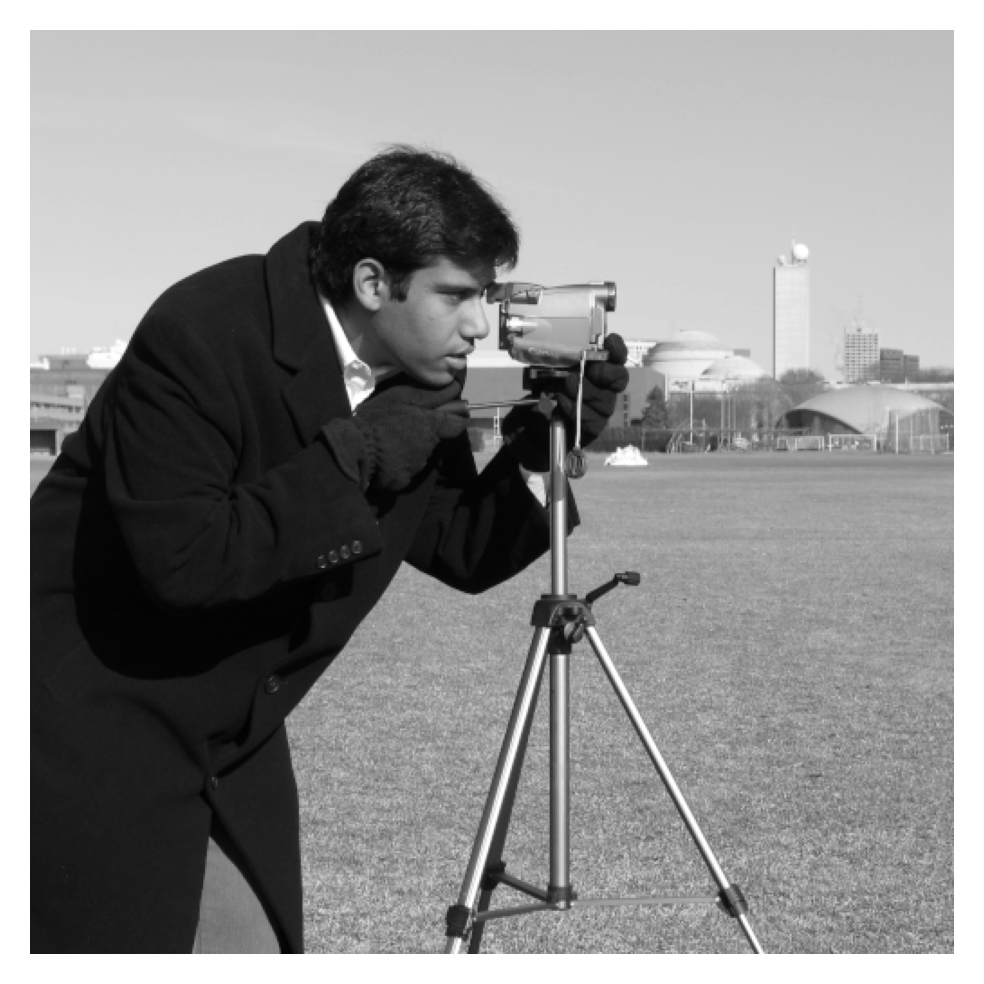
\includegraphics[height=.75\textheight]{data/camera}

  How to compress this image ?
\end{frame}

\begin{frame}{Low-rank approximation}
    \vfill

    \Large
    \[
    \begin{aligned}
      \minimize_{\bm{X}} & \quad \| \bm{A} - \bm{X} \|_F^2 \\
      \subto & \quad \mathrm{rank~} \bm{X} = r
    \end{aligned}
    \]

    \vfill
\end{frame}

{
  \setbeamercolor{background canvas}{bg=white}
  \setbeamercolor{background canvas}{bg=white}
  \setbeamercolor{normal text}{fg=black}

  \usebeamercolor[fg]{normal text}

  \begin{frame}
    \vfill
    \centering

    \begin{tikzpicture}[>=stealth]
      \begin{axis}[
        xmin=0, xmax=520,
        ymode=log,
        xlabel={Rank}, ylabel={$\sigma_i$},
        width=\textwidth,
        height=.66\textheight,
        axis lines = middle,
        y axis line style={stealth-},
        x label style={at={(axis description cs:0.5, 1.05)}, anchor=south},
        y label style={at={(axis description cs:0, 0)}, anchor=north east},
        ]

        % --> Plot singular spectrum.
        \addplot[ultra thick, orange, smooth] table[x=x, y=y]{data/camera_svd.dat};

      \end{axis}
    \end{tikzpicture}

    \vfill
  \end{frame}


  \begin{frame}
    \vfill
    \centering

    \begin{tikzpicture}[>=stealth]
      \begin{axis}[
          xmin=0, xmax=520,
          ymin=0, ymax=1.1,
          xlabel={Rank}, ylabel={Cumulative sum},
          width=\textwidth,
          height=.66\textheight,
          axis lines = middle,
          x label style={at={(axis description cs:0.5, -0.2)}, anchor=north},
          y label style={at={(axis description cs:-0.075, 0.5)}, rotate=90, anchor=south},
        ]

        % --> Plot singular spectrum.
        \addplot[ultra thick, orange, smooth] table[x=x, y=y]{data/camera_svd_bis.dat};

        \addplot[mark=none, black, dashed] coordinates {(0, 1) (520, 1)};

      \end{axis}
    \end{tikzpicture}

    \vfill
  \end{frame}


}

\begin{frame}%{Low-rank approximation}
  \centering
  \vfill

  
\includegraphics[width=.15\textwidth]{camera_svd_1_comp}%
  \hfill
  
\includegraphics[width=.15\textwidth]{camera_svd_2_comp}%
  \hfill
  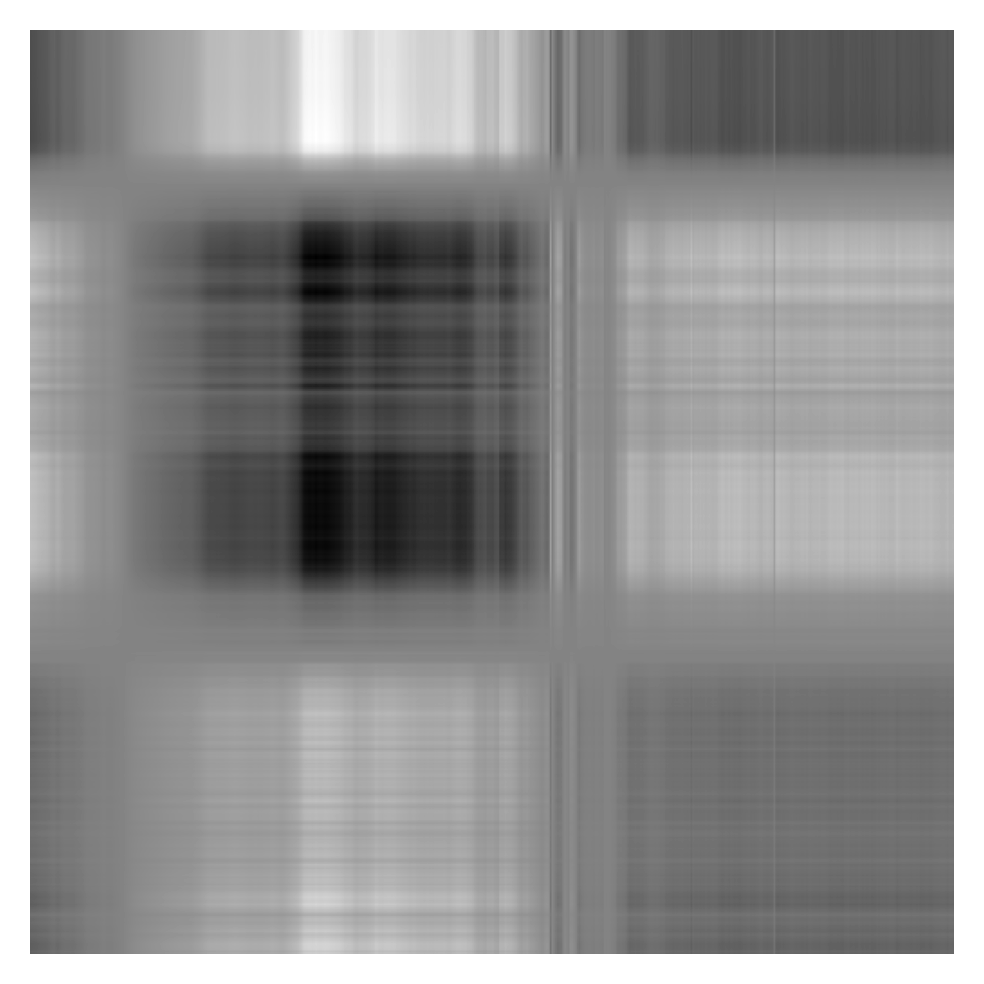
\includegraphics[width=.15\textwidth]{camera_svd_3_comp}%
  \hfill
  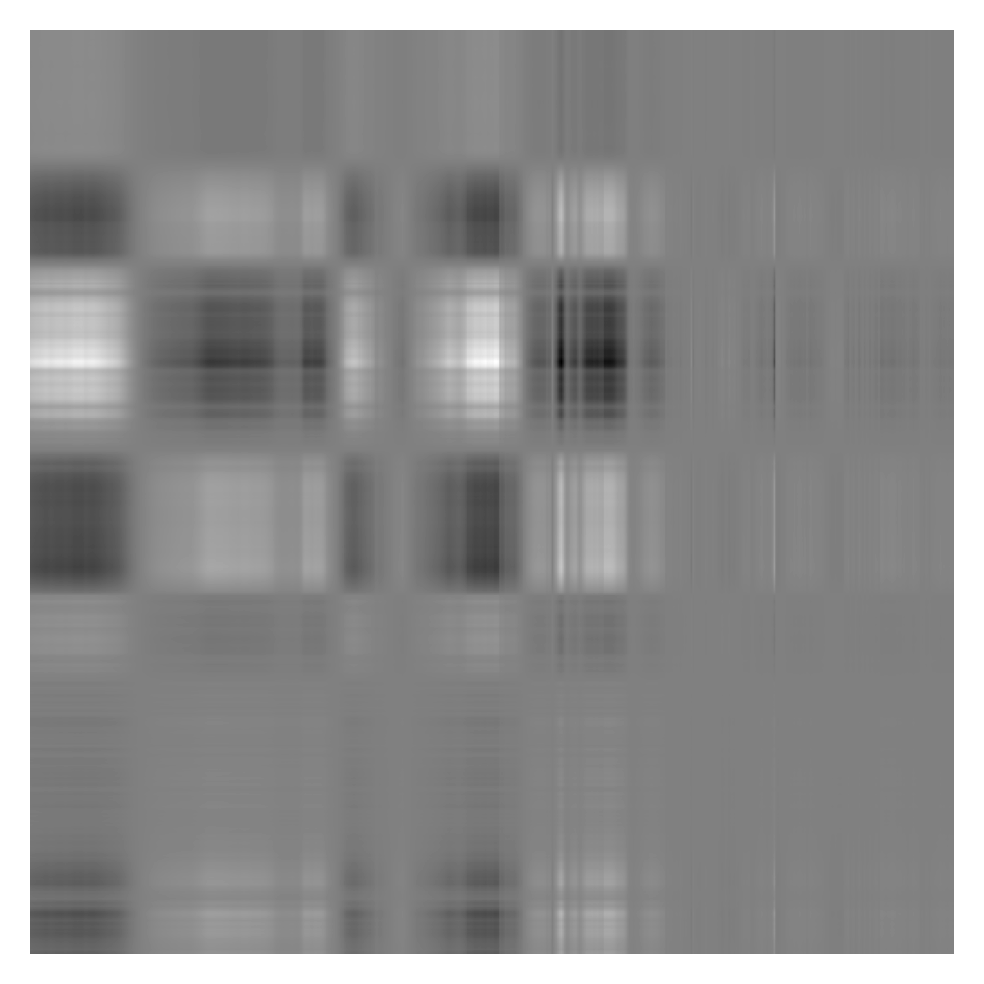
\includegraphics[width=.15\textwidth]{camera_svd_4_comp}%
  \hfill
  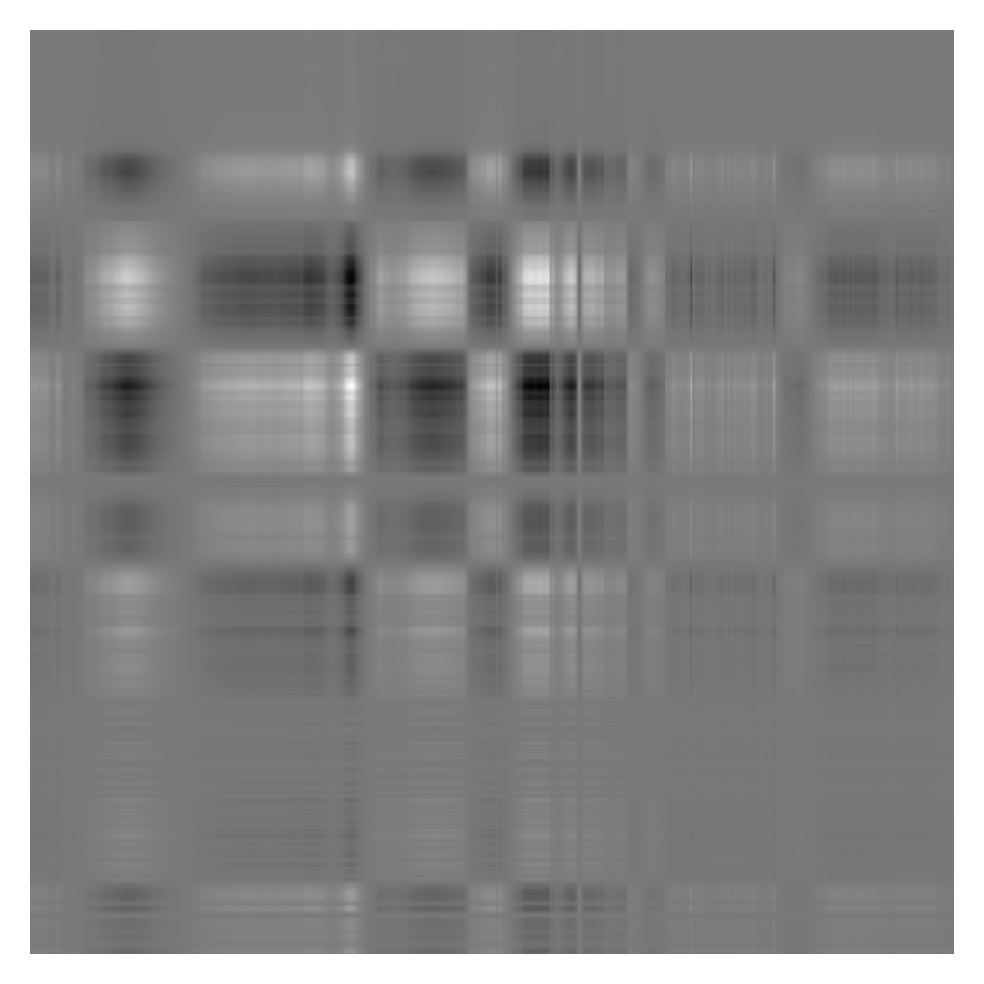
\includegraphics[width=.15\textwidth]{camera_svd_5_comp}%
  \hfill
  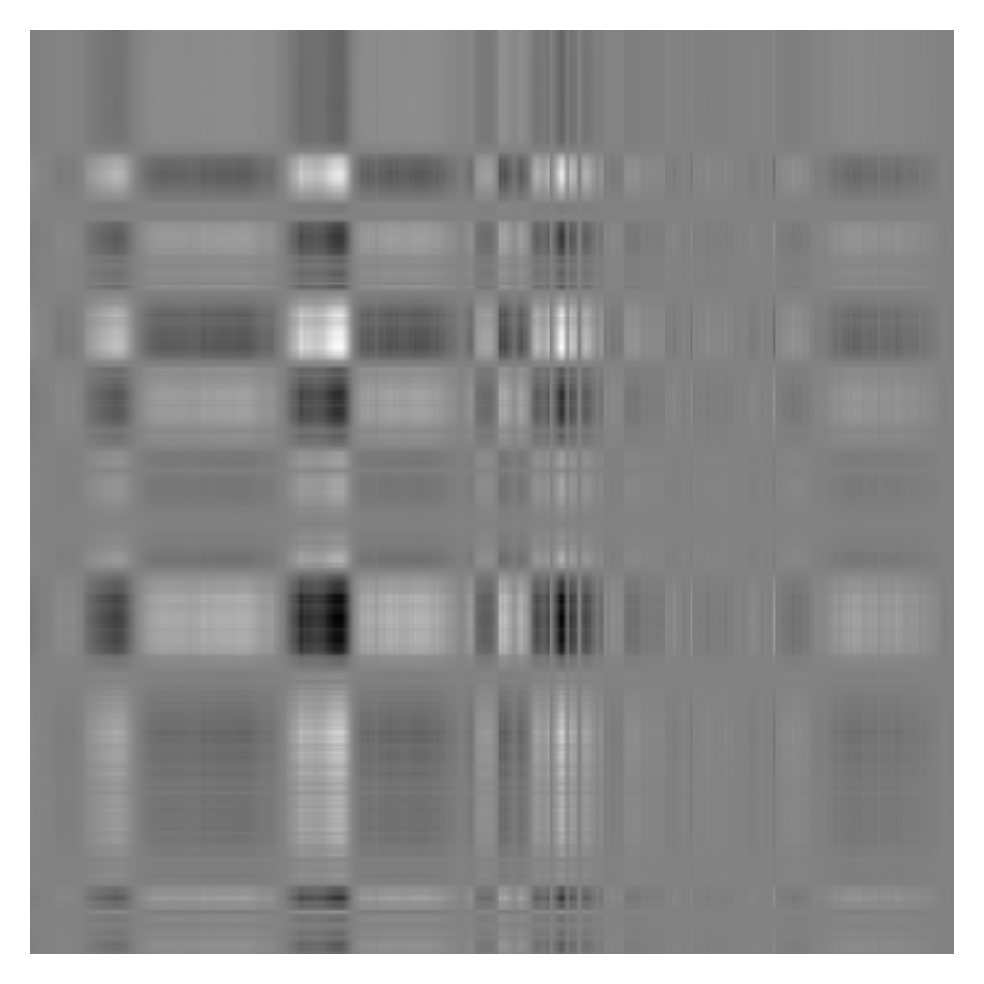
\includegraphics[width=.15\textwidth]{camera_svd_6_comp}

  \vfill

  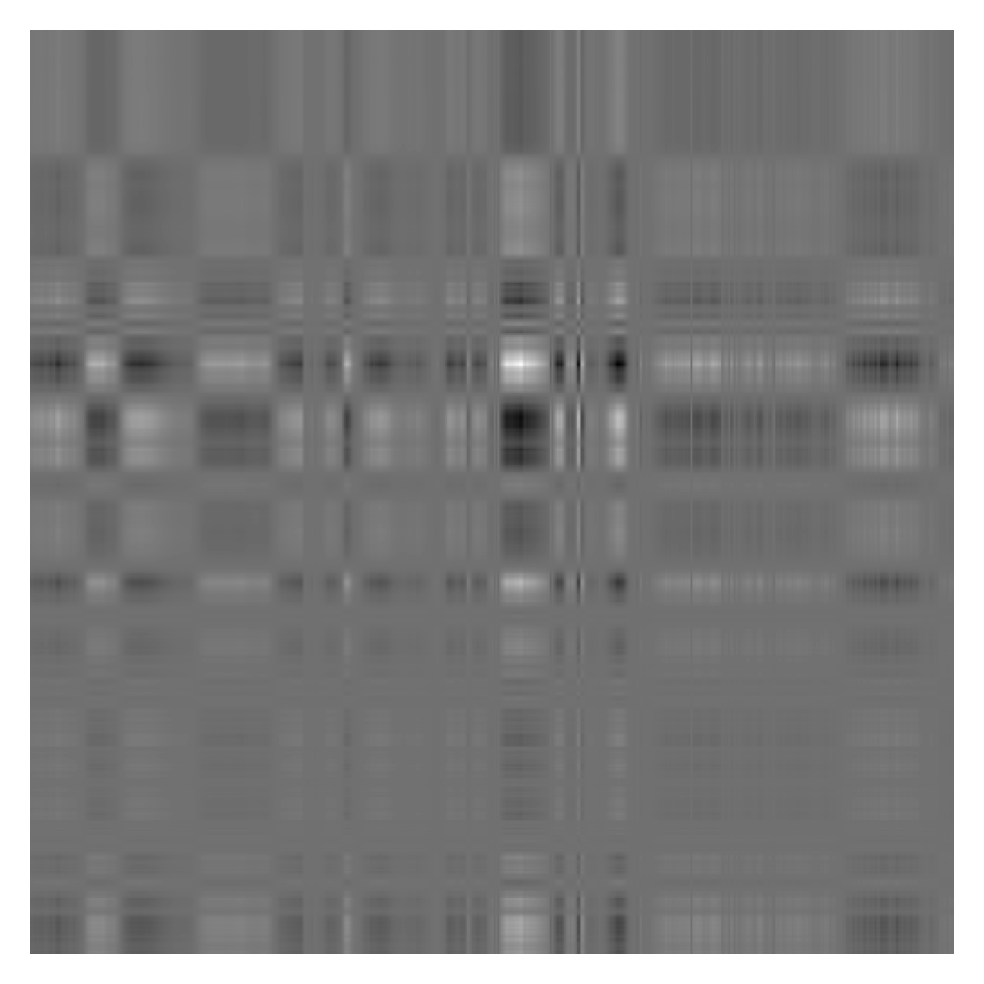
\includegraphics[width=.15\textwidth]{camera_svd_7_comp}%
  \hfill
  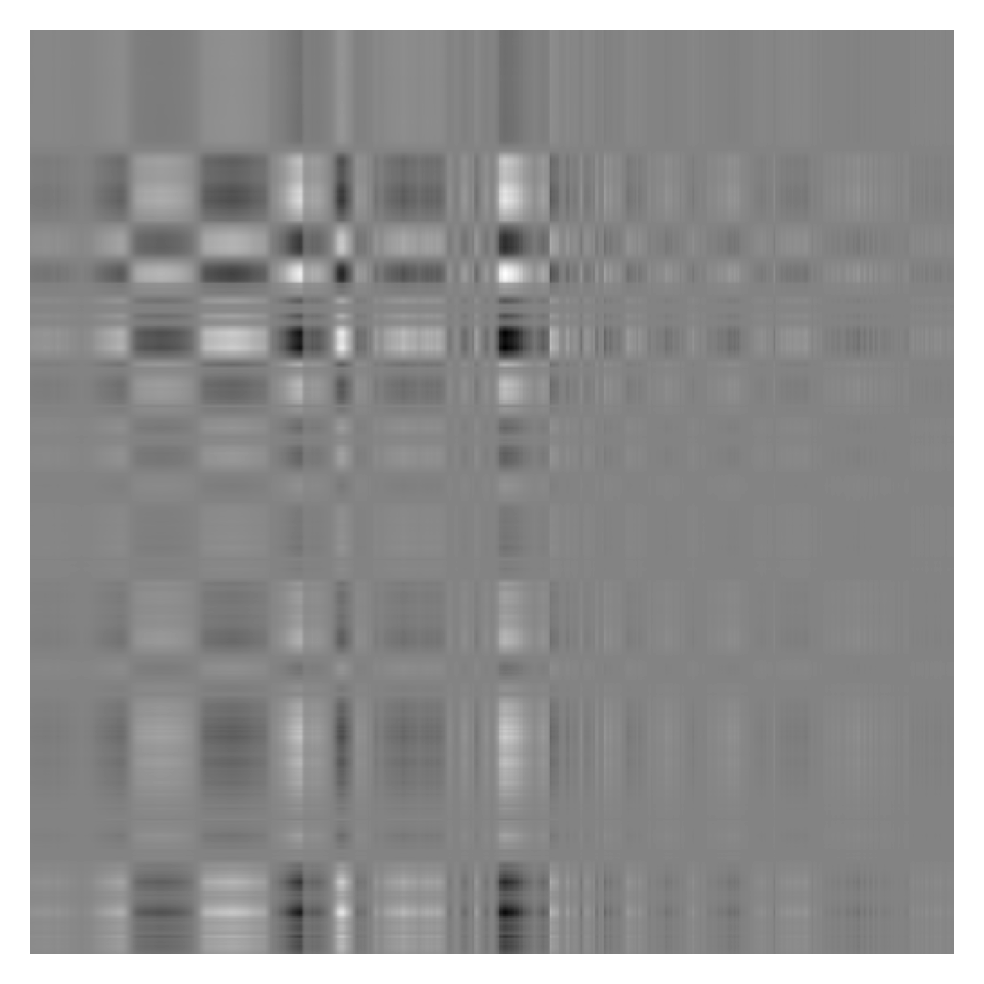
\includegraphics[width=.15\textwidth]{camera_svd_8_comp}%
  \hfill
  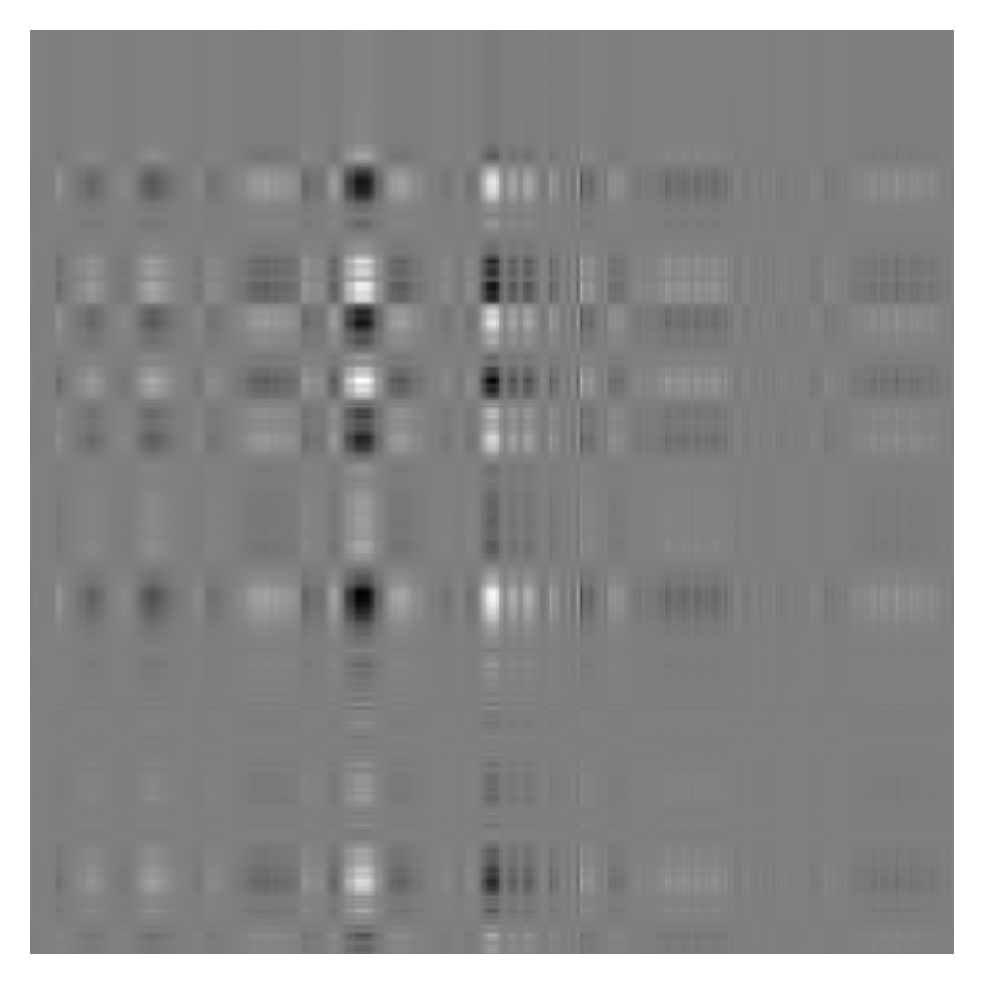
\includegraphics[width=.15\textwidth]{camera_svd_9_comp}%
  \hfill
  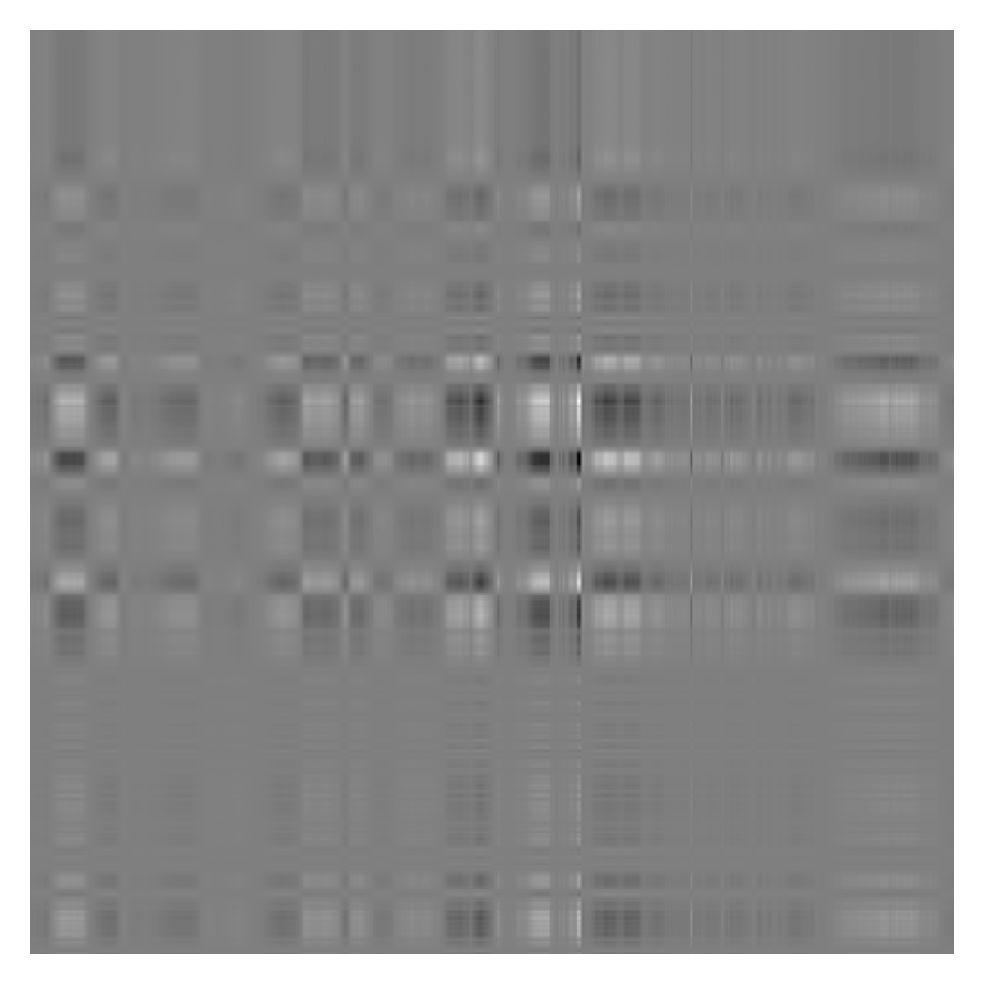
\includegraphics[width=.15\textwidth]{camera_svd_10_comp}%
  \hfill
  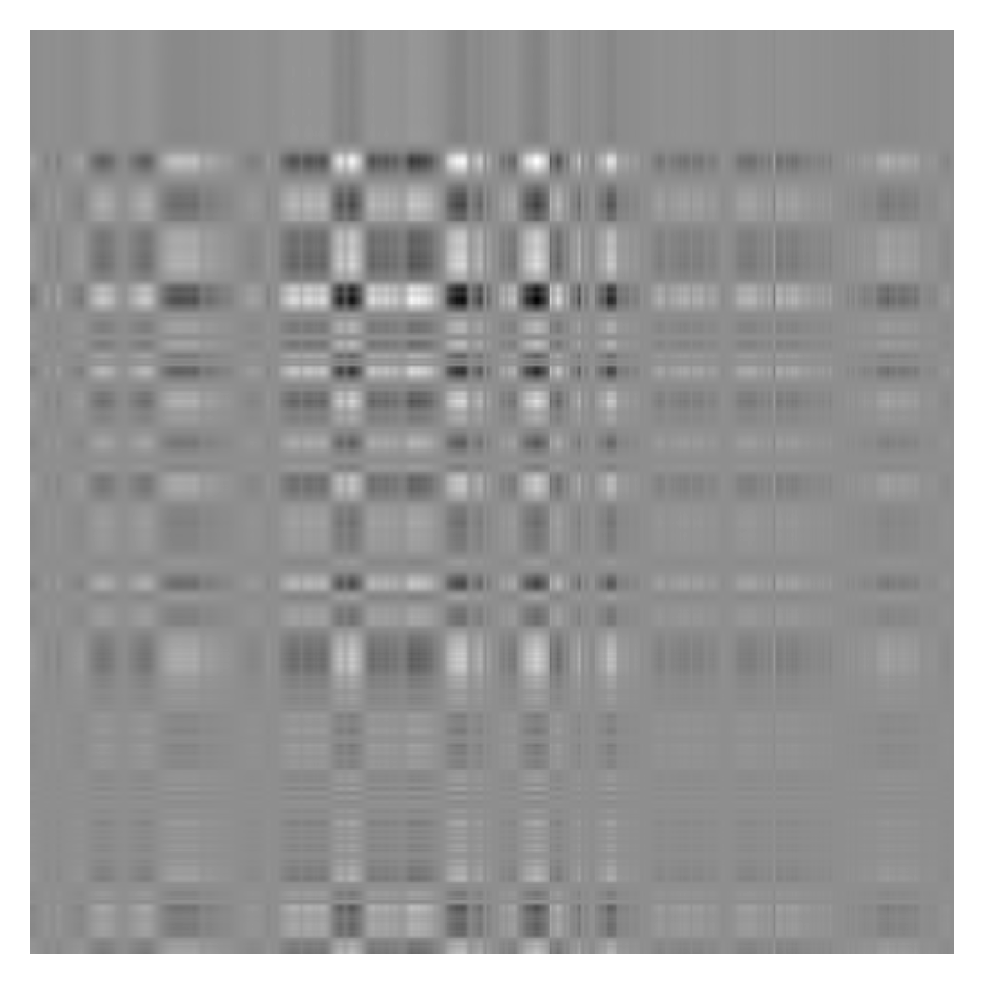
\includegraphics[width=.15\textwidth]{camera_svd_11_comp}%
  \hfill
  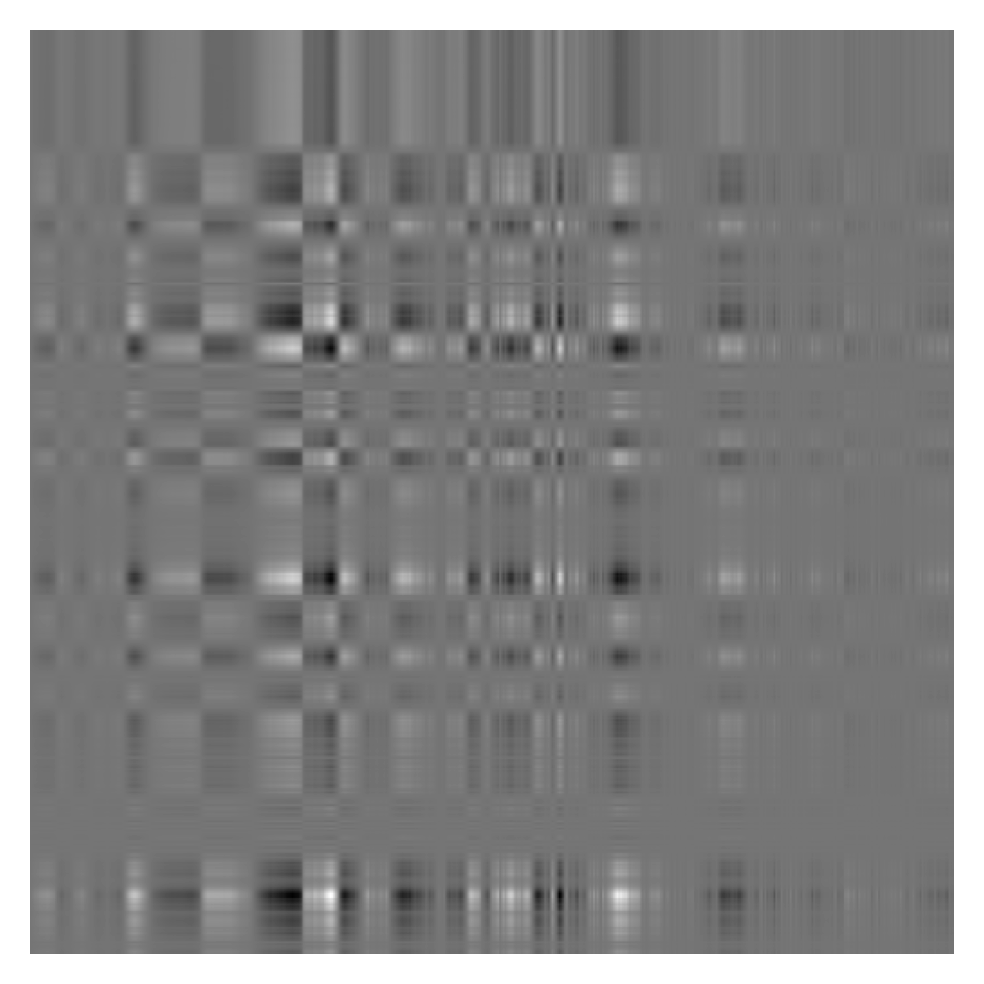
\includegraphics[width=.15\textwidth]{camera_svd_12_comp}

  \vfill

  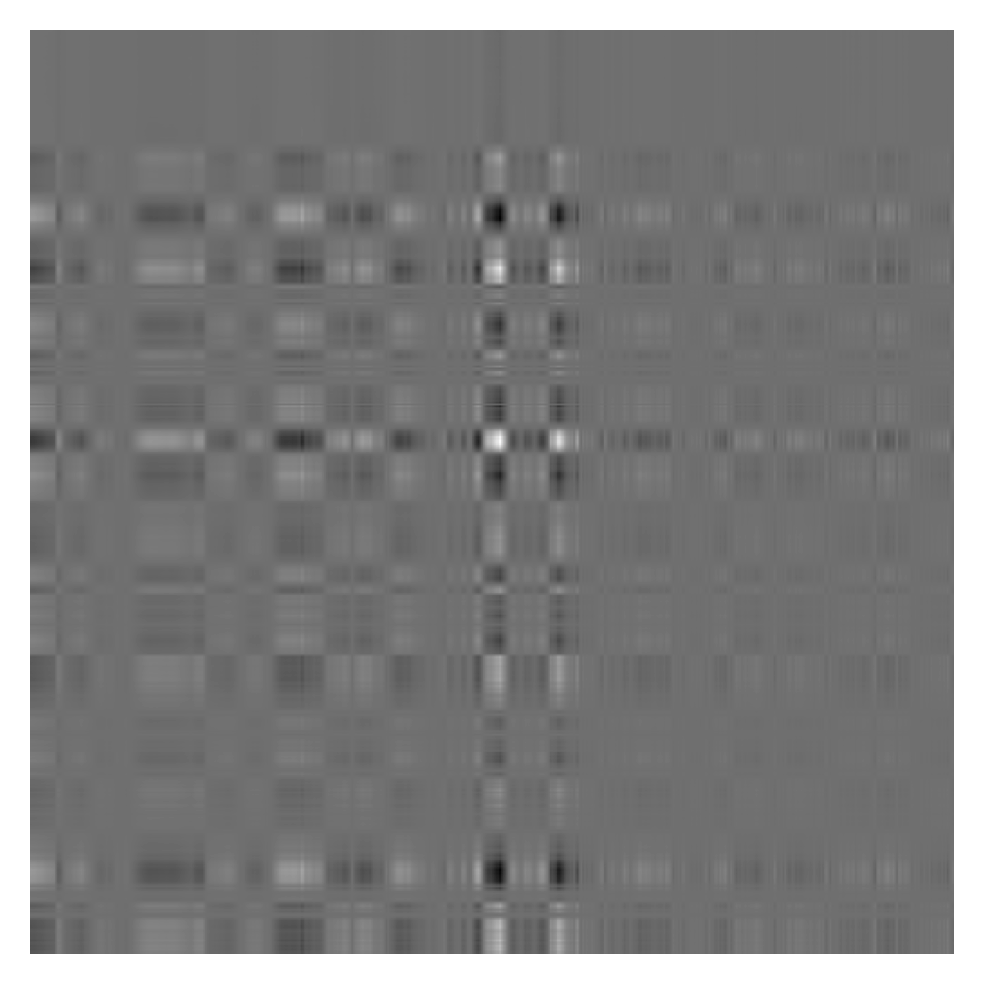
\includegraphics[width=.15\textwidth]{camera_svd_13_comp}%
  \hfill
  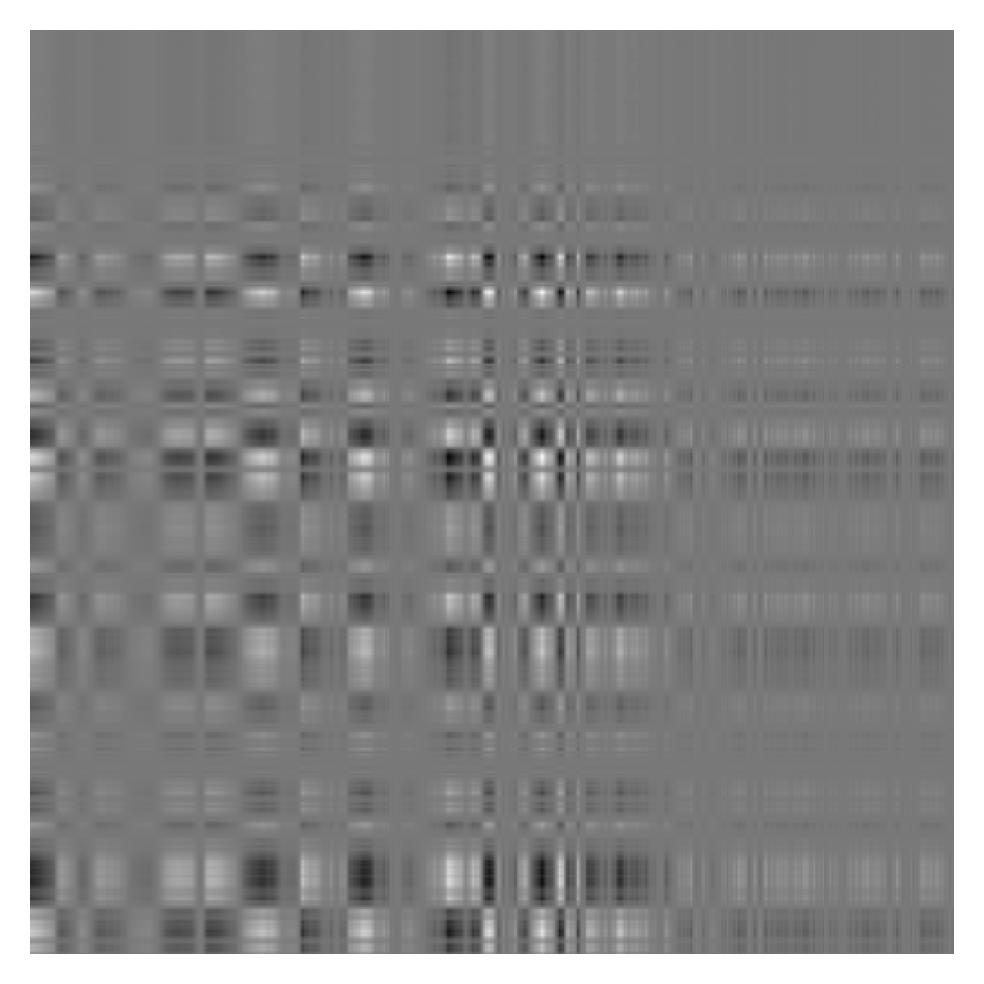
\includegraphics[width=.15\textwidth]{camera_svd_14_comp}%
  \hfill
  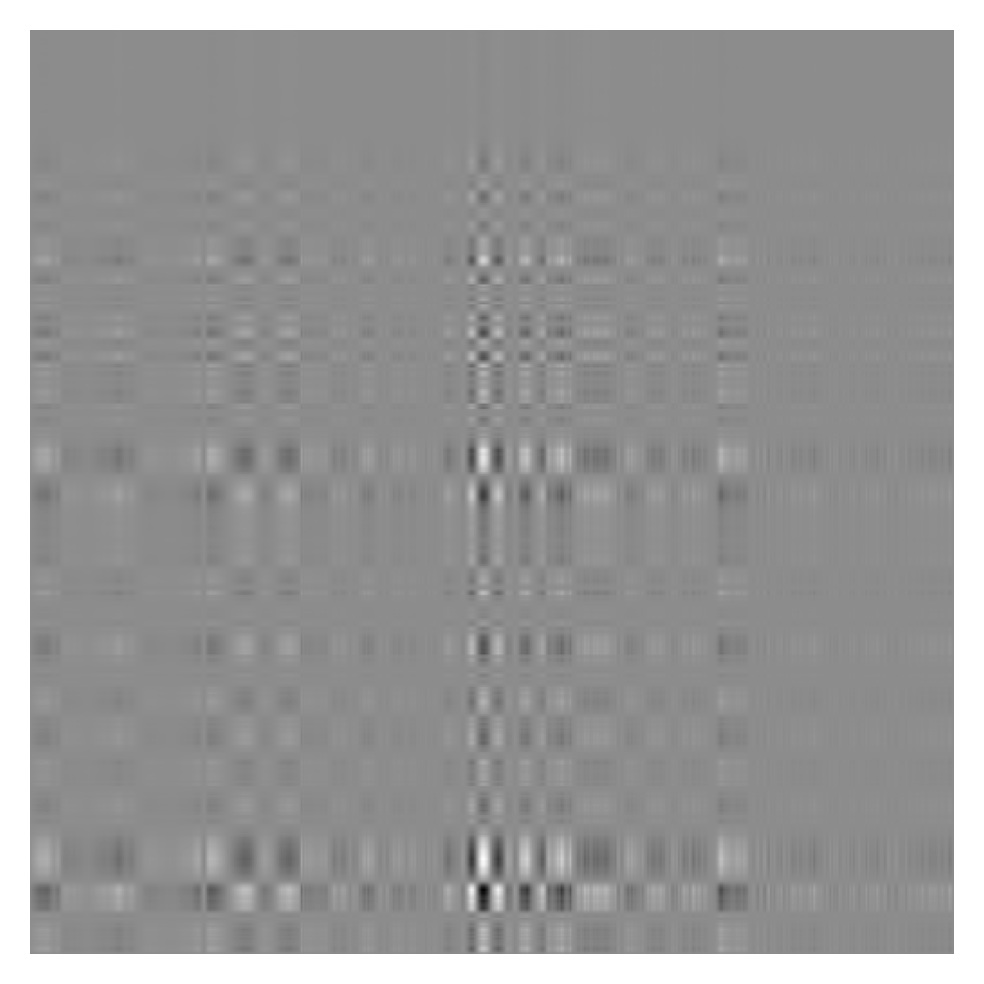
\includegraphics[width=.15\textwidth]{camera_svd_15_comp}%
  \hfill
  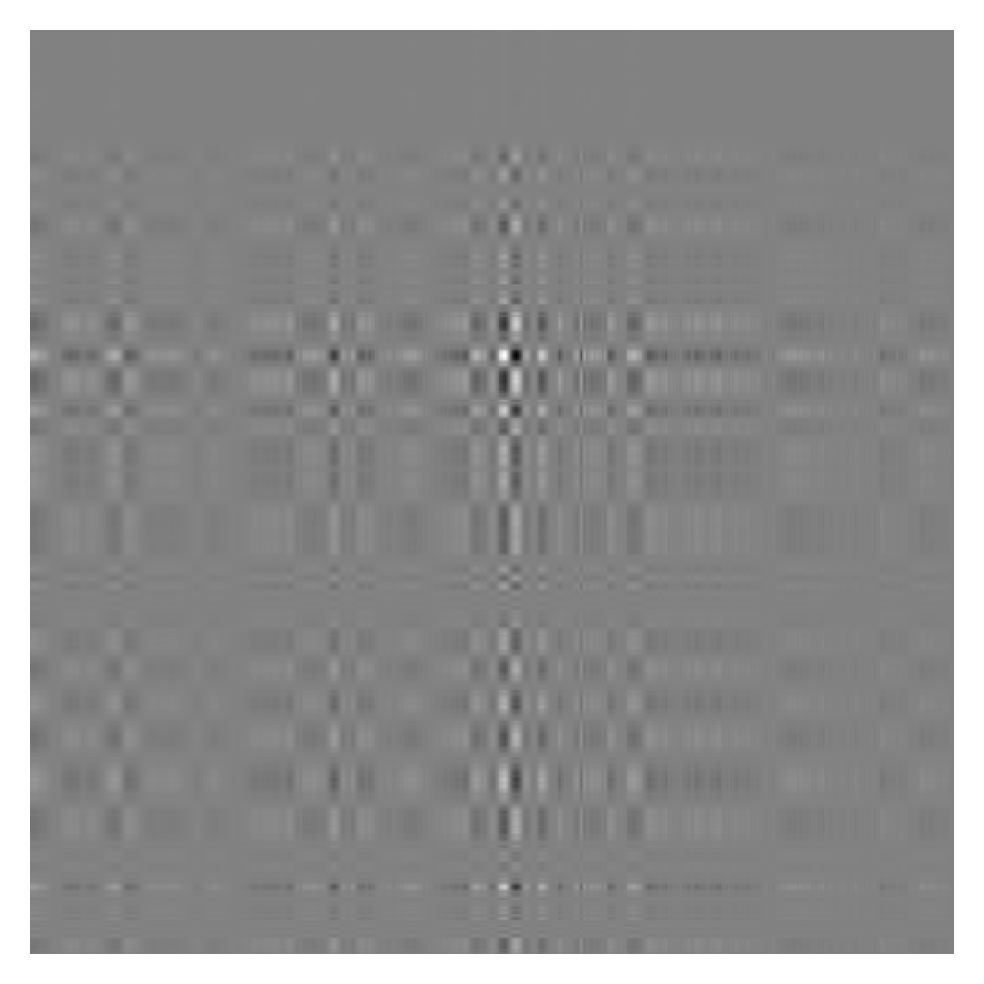
\includegraphics[width=.15\textwidth]{camera_svd_16_comp}%
  \hfill
  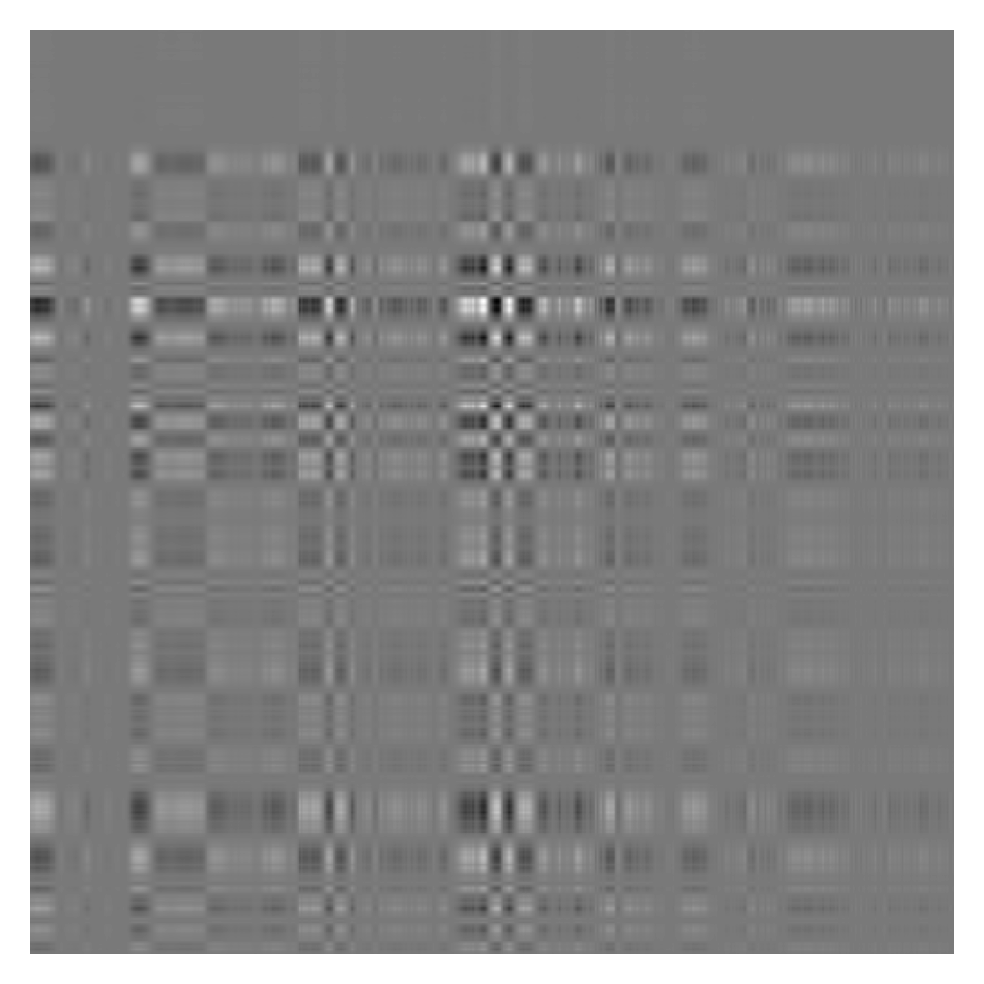
\includegraphics[width=.15\textwidth]{camera_svd_17_comp}%
  \hfill
  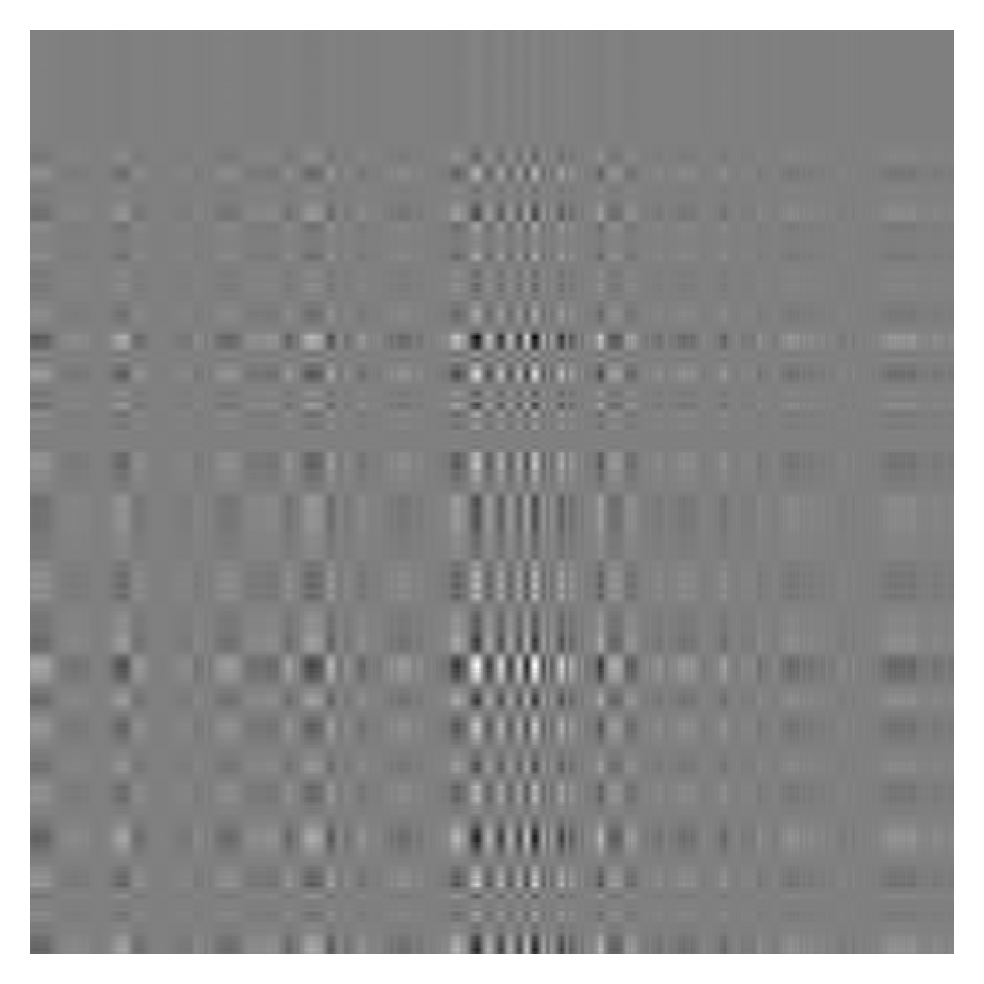
\includegraphics[width=.15\textwidth]{camera_svd_18_comp}

  \vfill
\end{frame}

\begin{frame}%{Low-rank approximation}
  \centering
  \vfill

  
\includegraphics[width=.15\textwidth]{camera_svd_1_estimate}%
  \hfill
  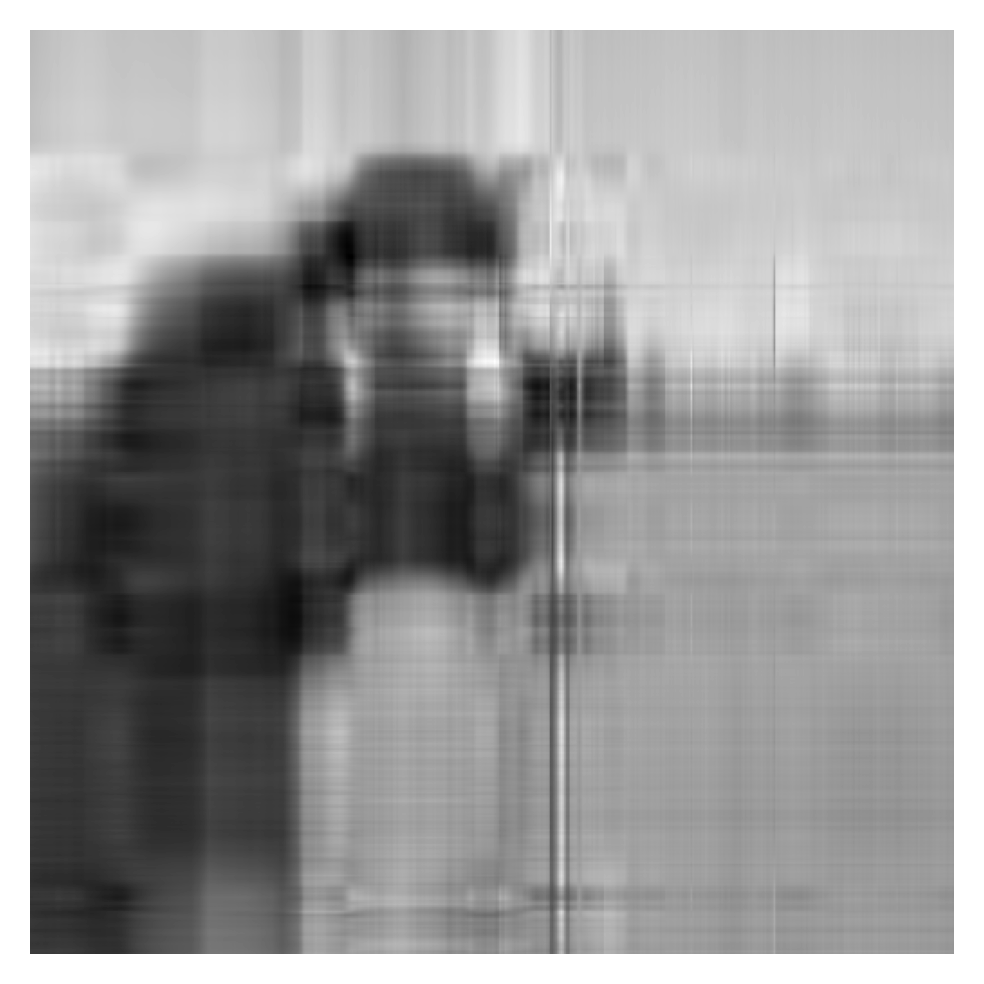
\includegraphics[width=.15\textwidth]{camera_svd_6_estimate}%
  \hfill
  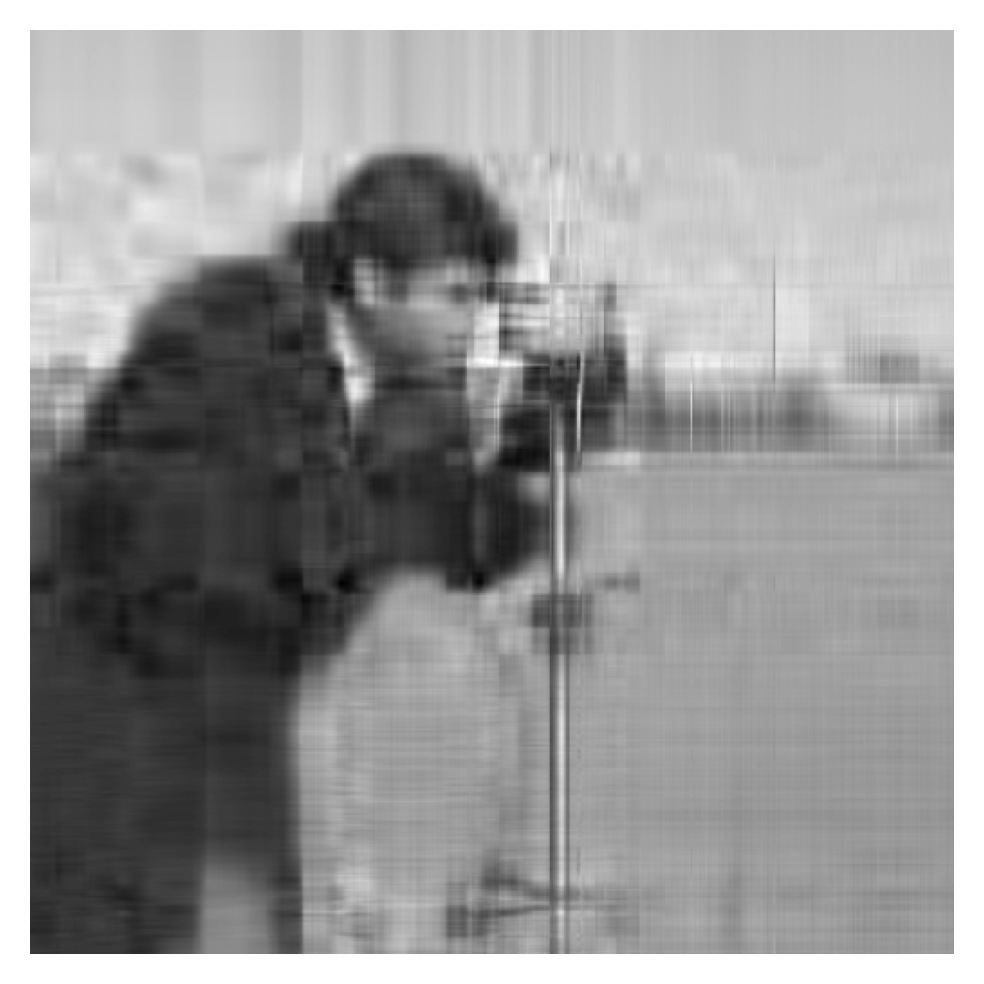
\includegraphics[width=.15\textwidth]{camera_svd_11_estimate}%
  \hfill
  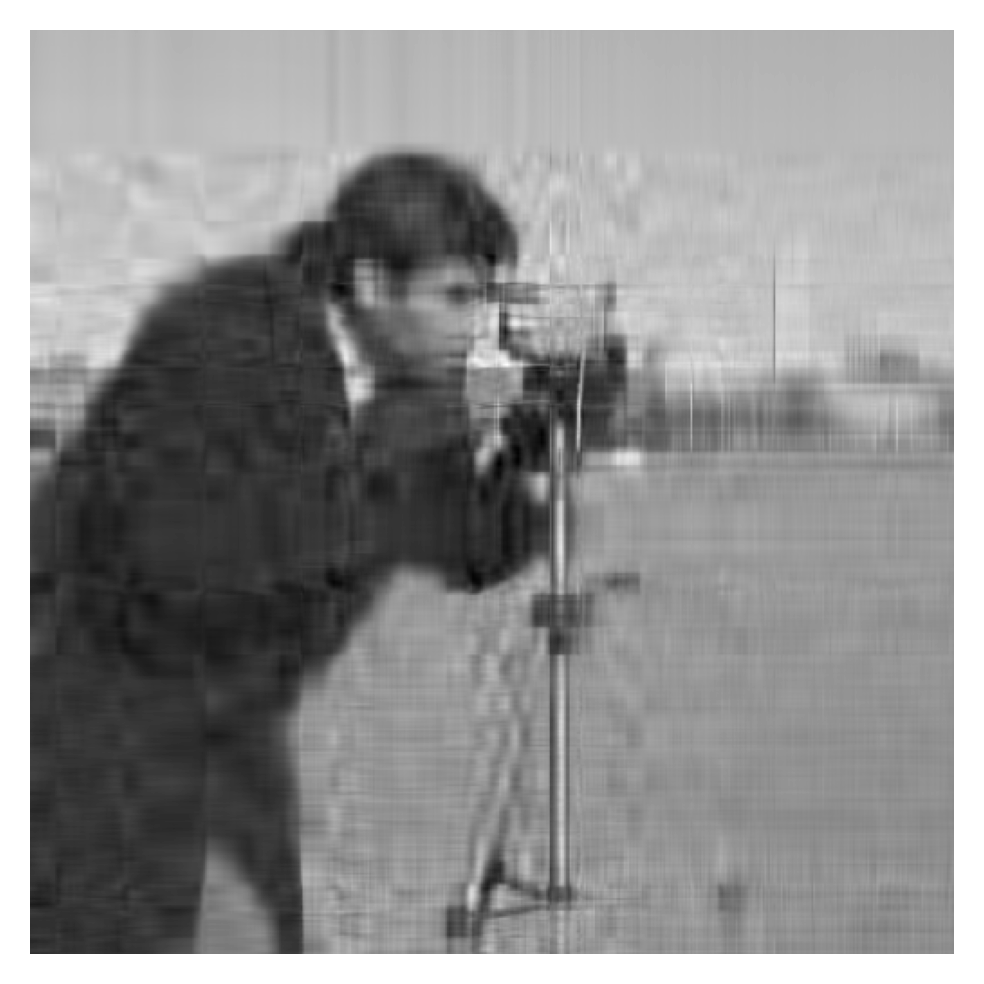
\includegraphics[width=.15\textwidth]{camera_svd_16_estimate}%
  \hfill
  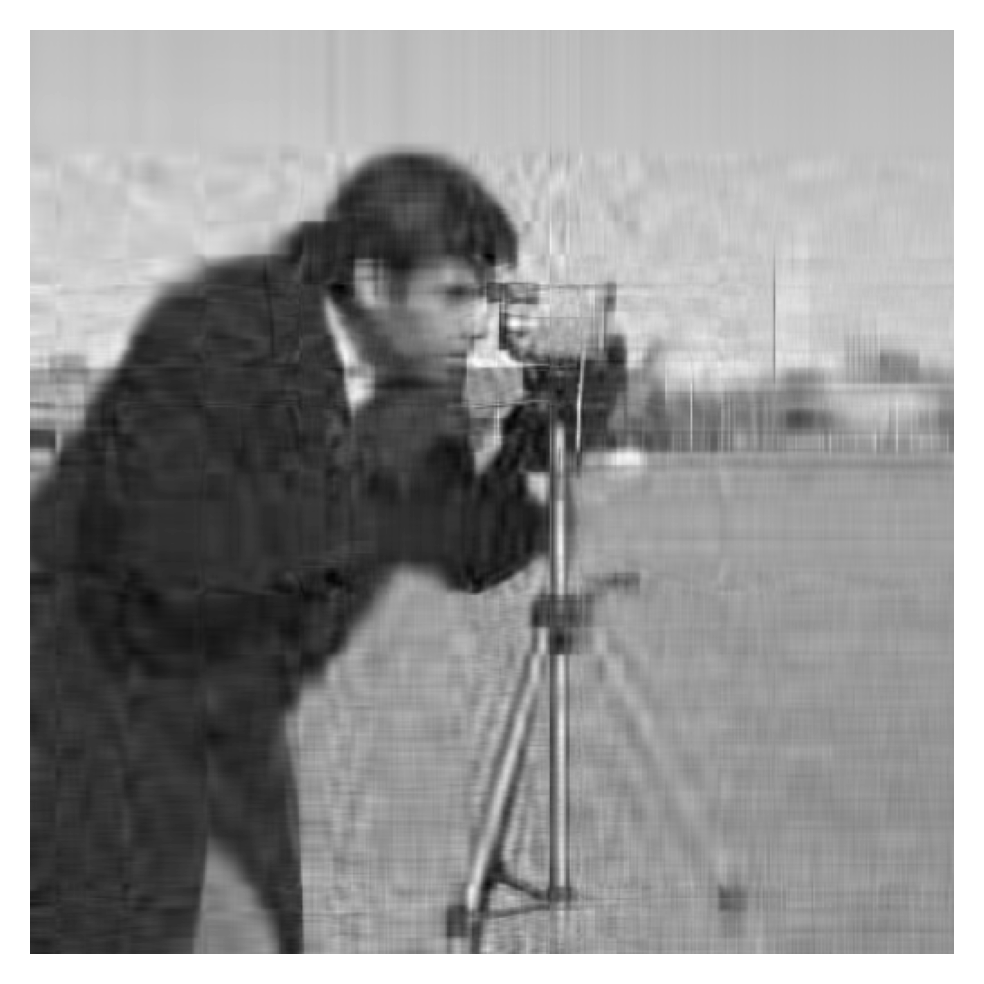
\includegraphics[width=.15\textwidth]{camera_svd_21_estimate}%
  \hfill
  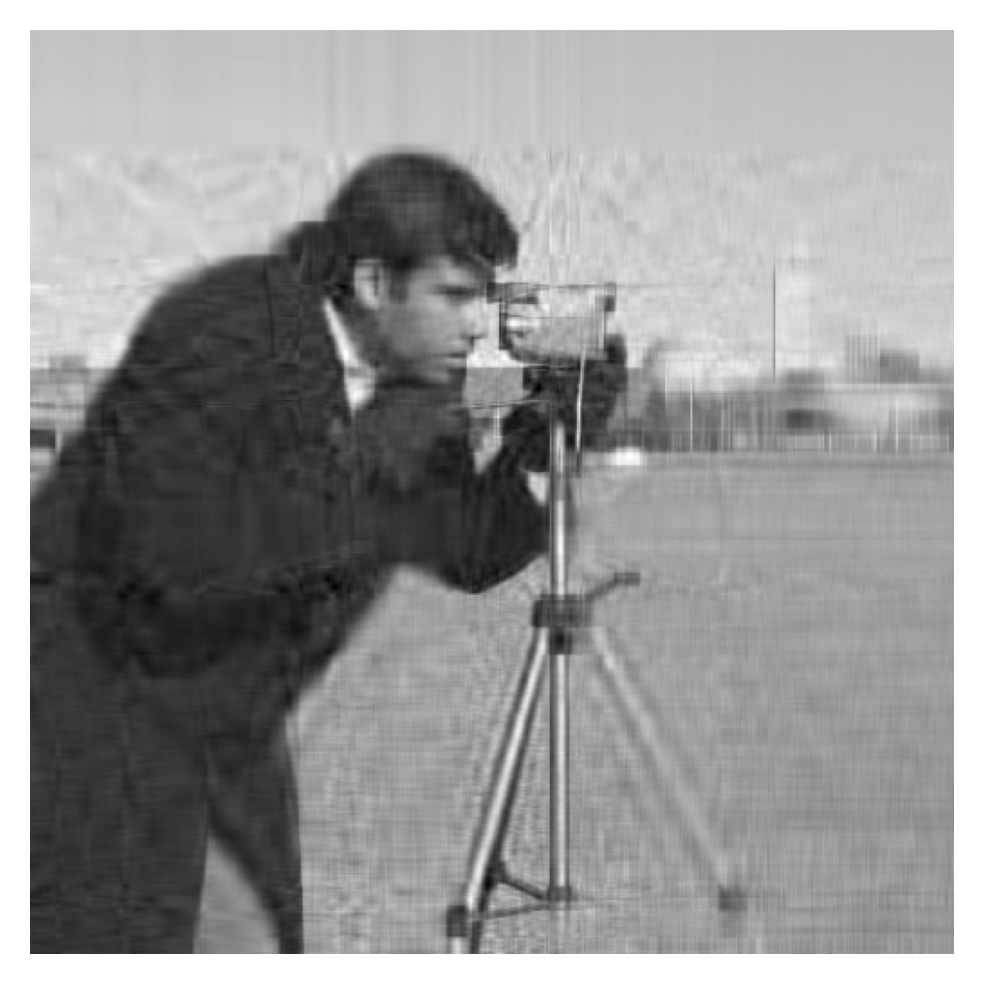
\includegraphics[width=.15\textwidth]{camera_svd_26_estimate}

  \vfill

  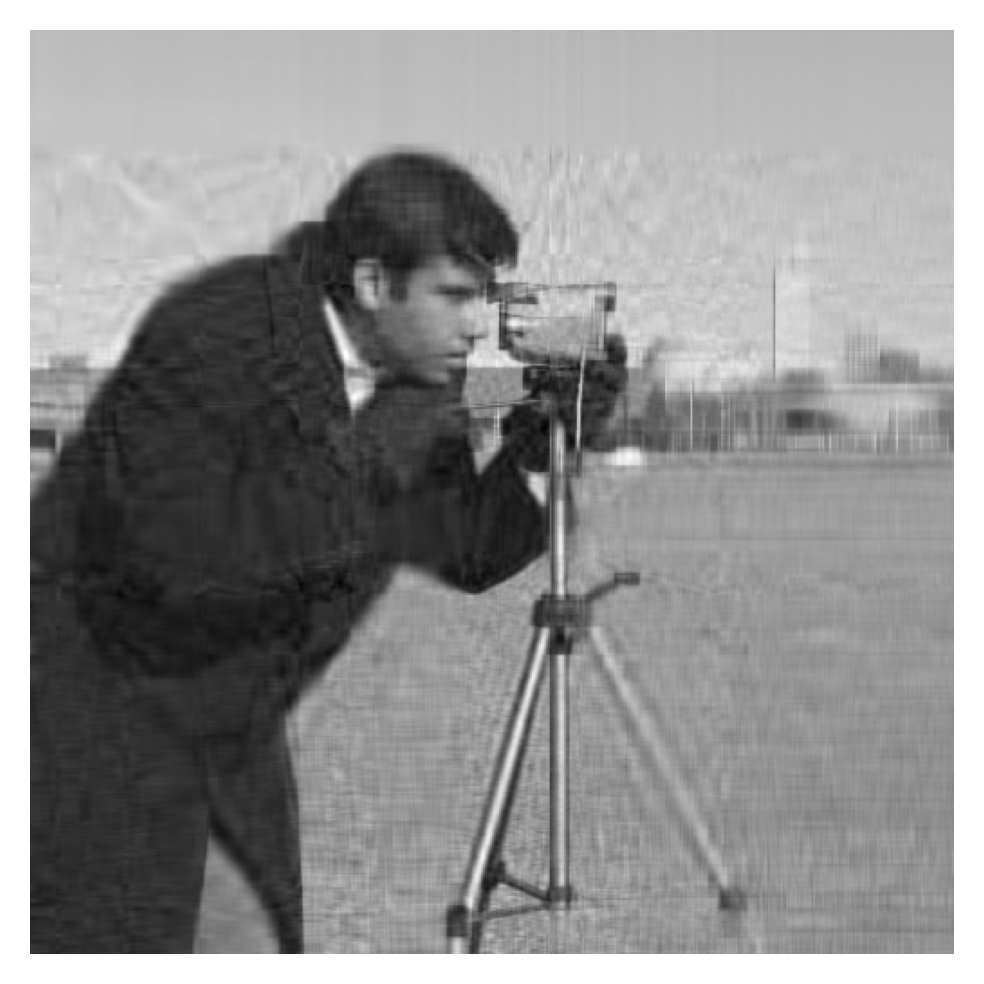
\includegraphics[width=.15\textwidth]{camera_svd_31_estimate}%
  \hfill
  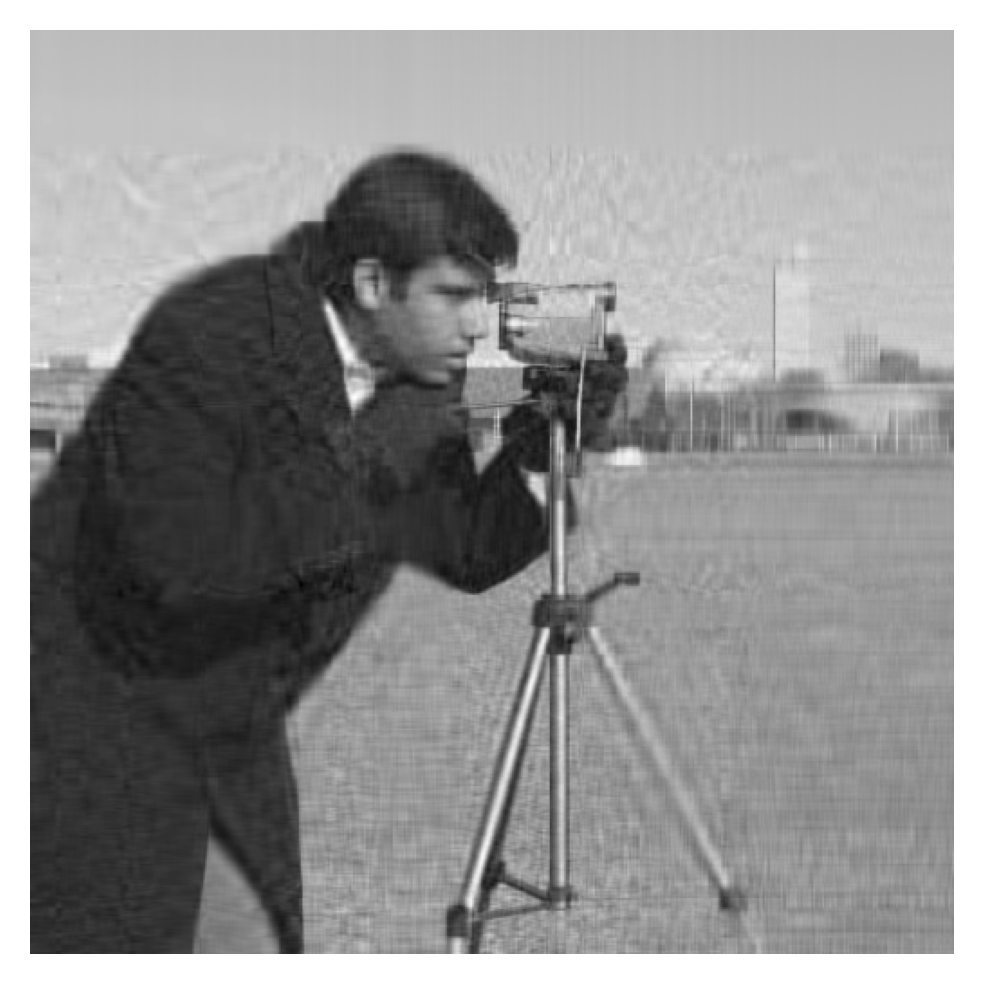
\includegraphics[width=.15\textwidth]{camera_svd_36_estimate}%
  \hfill
  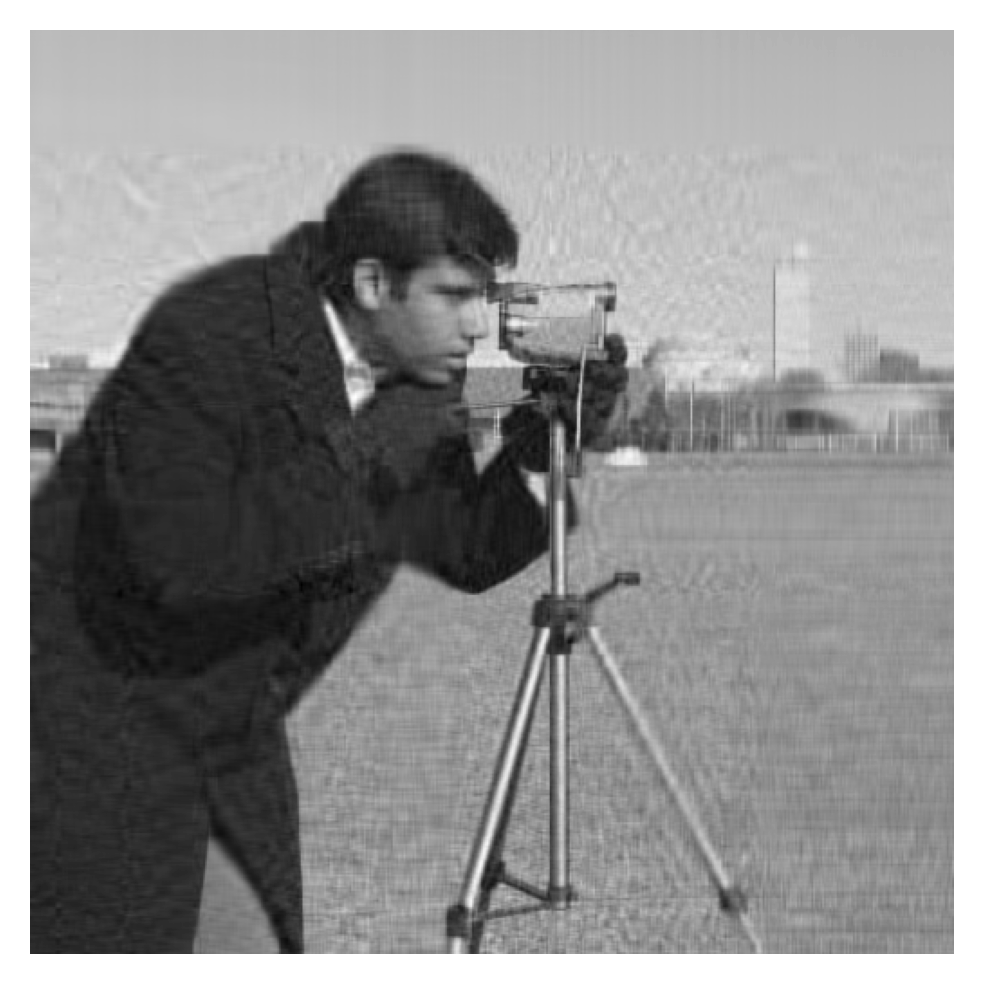
\includegraphics[width=.15\textwidth]{camera_svd_41_estimate}%
  \hfill
  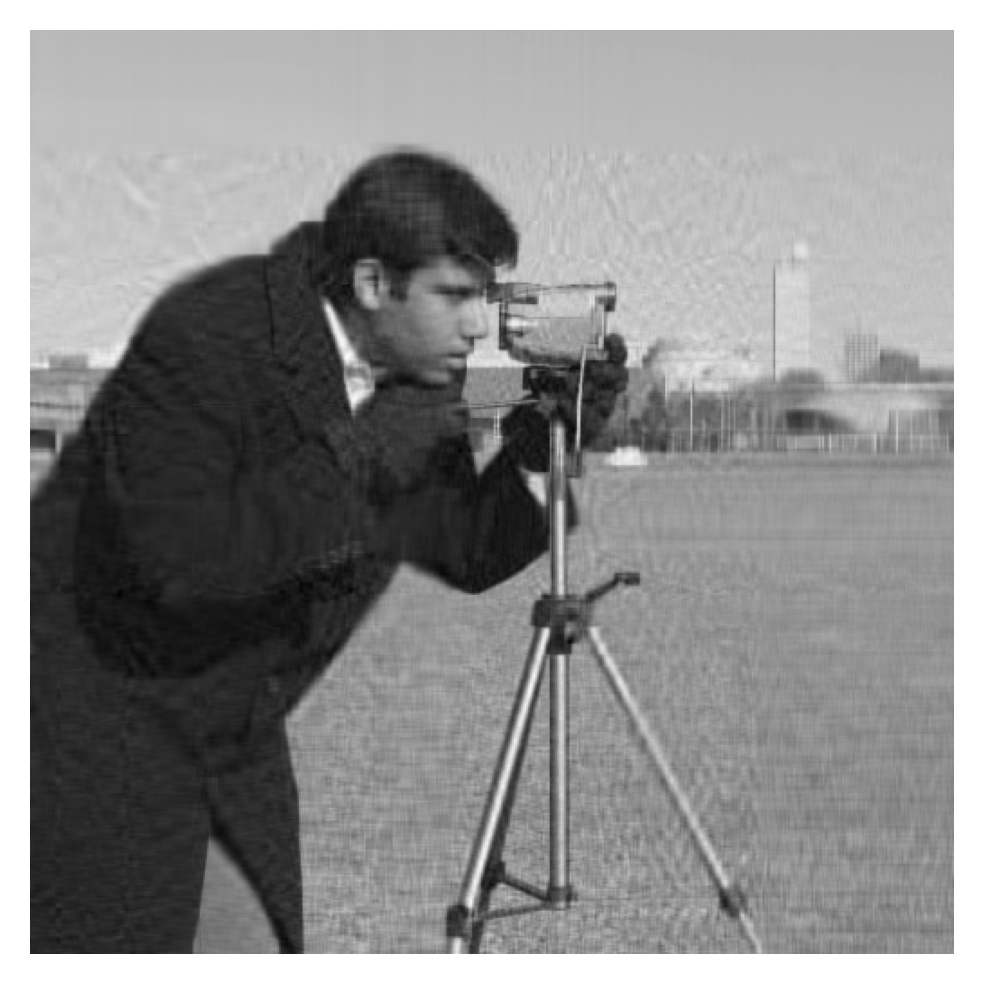
\includegraphics[width=.15\textwidth]{camera_svd_46_estimate}%
  \hfill
  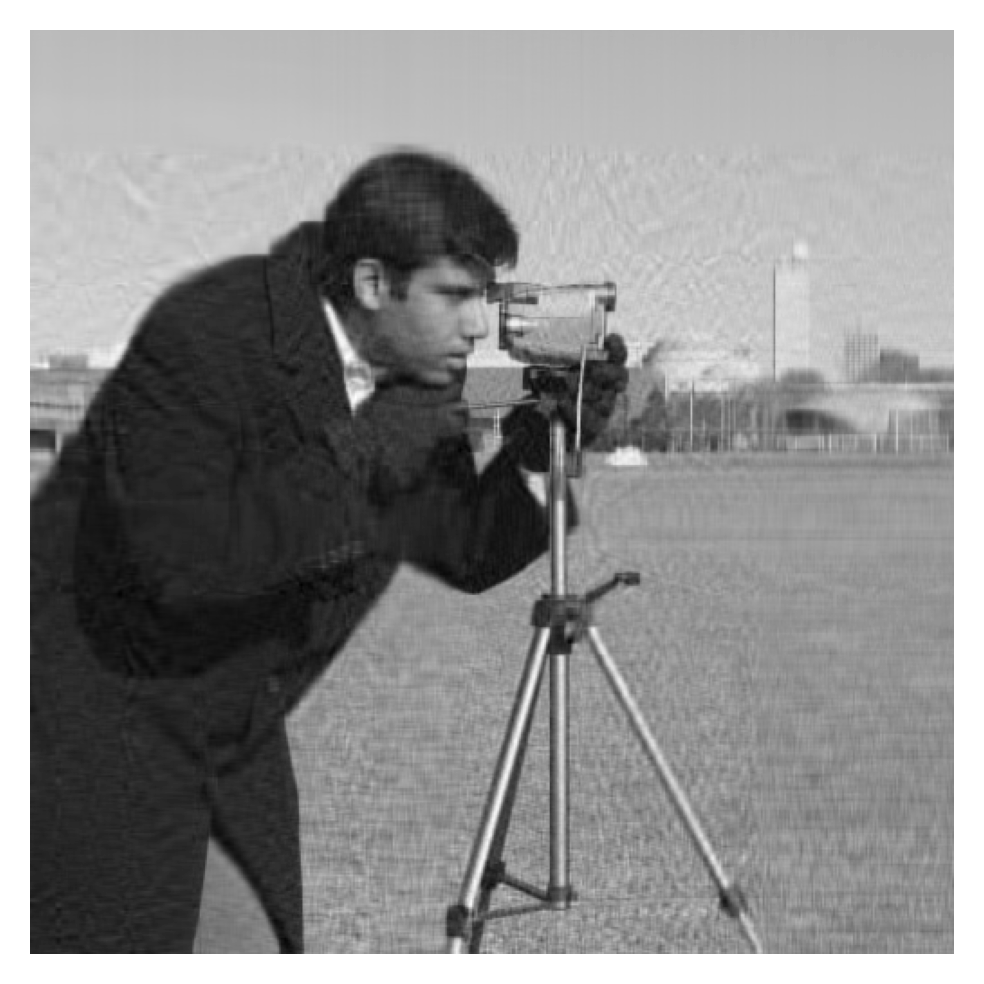
\includegraphics[width=.15\textwidth]{camera_svd_51_estimate}%
  \hfill
  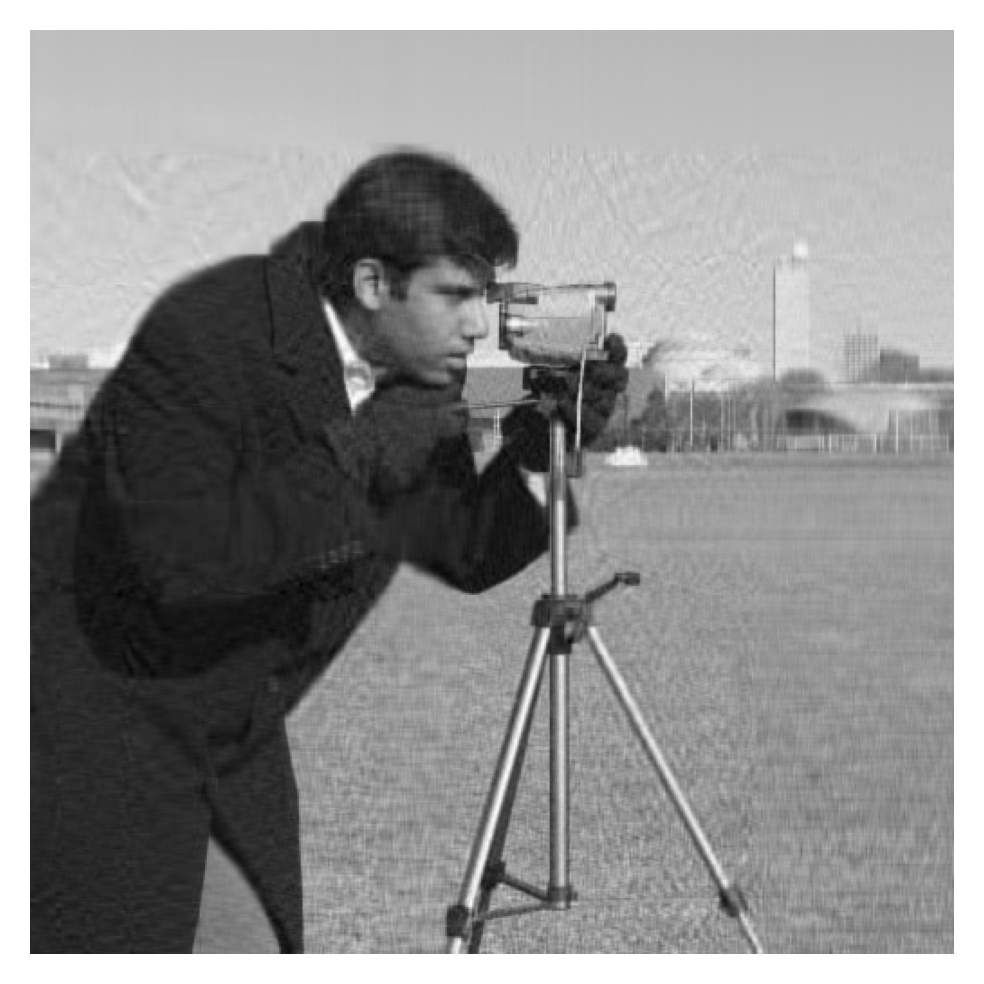
\includegraphics[width=.15\textwidth]{camera_svd_56_estimate}

  \vfill

  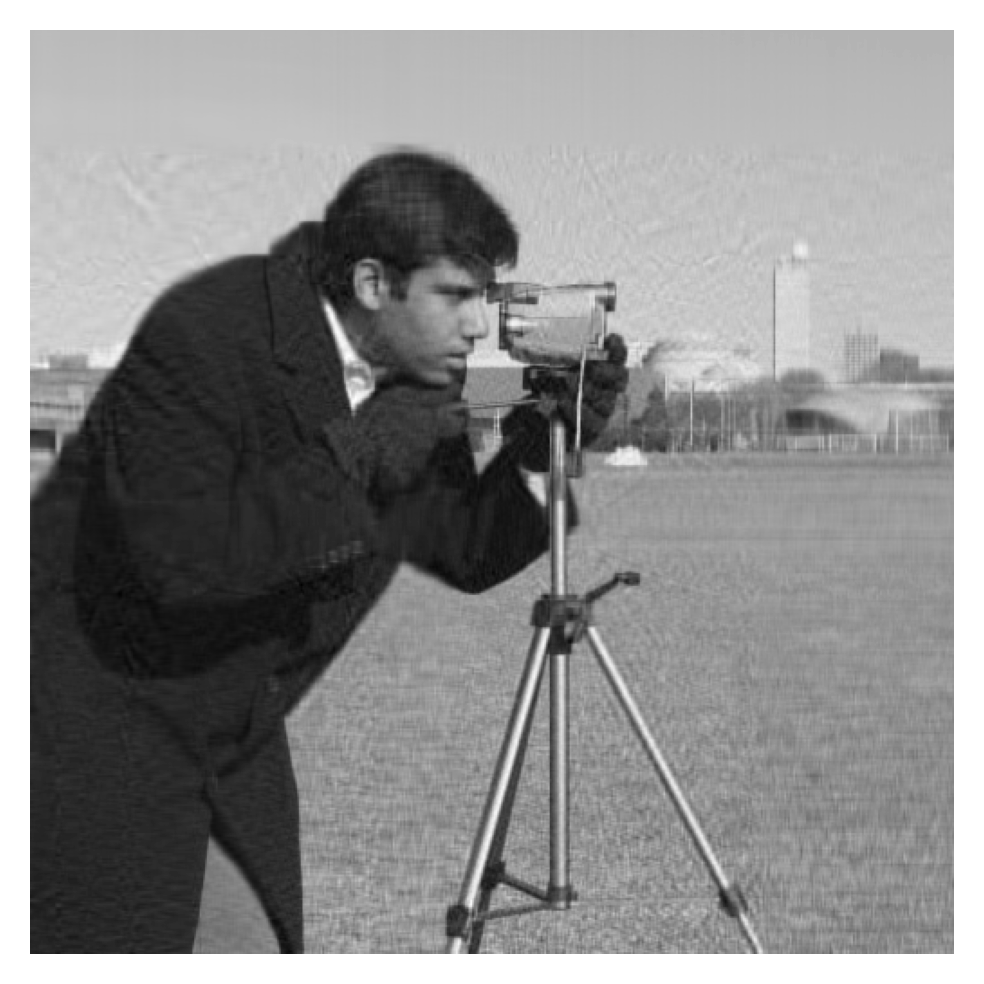
\includegraphics[width=.15\textwidth]{camera_svd_61_estimate}%
  \hfill
  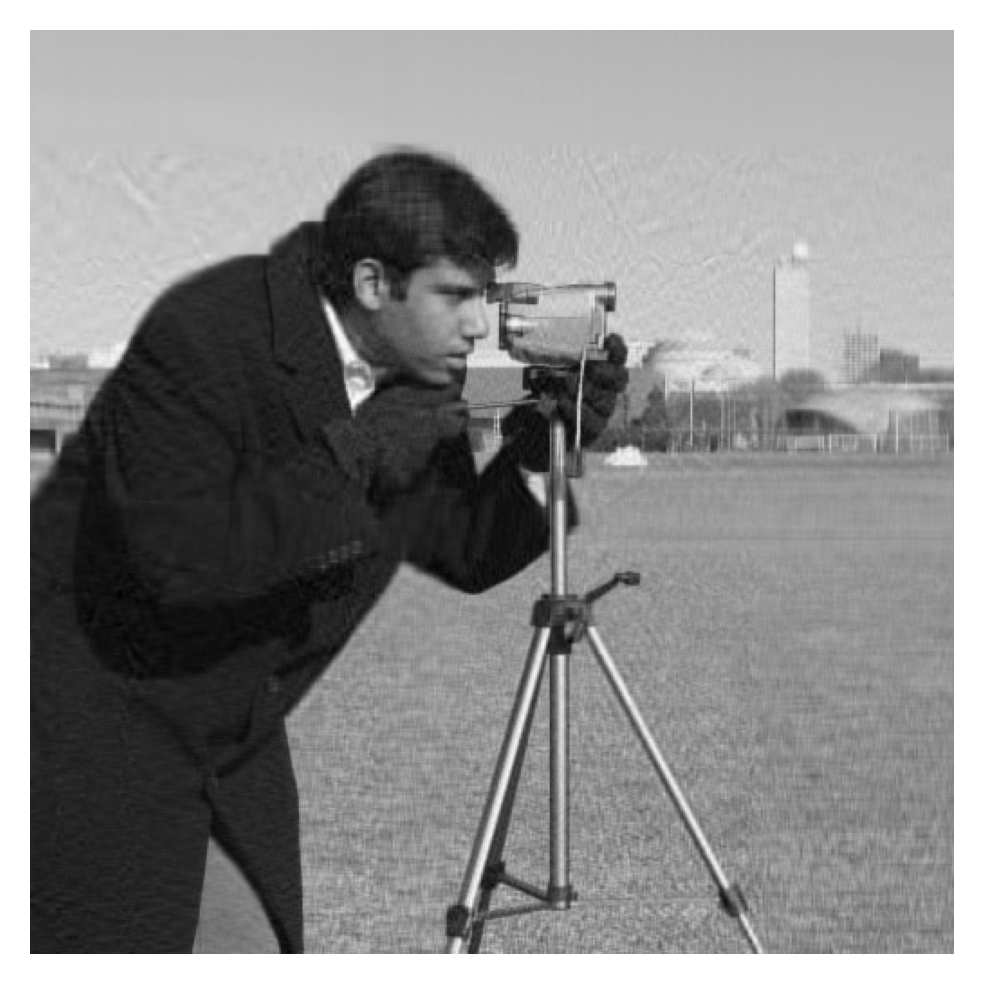
\includegraphics[width=.15\textwidth]{camera_svd_66_estimate}%
  \hfill
  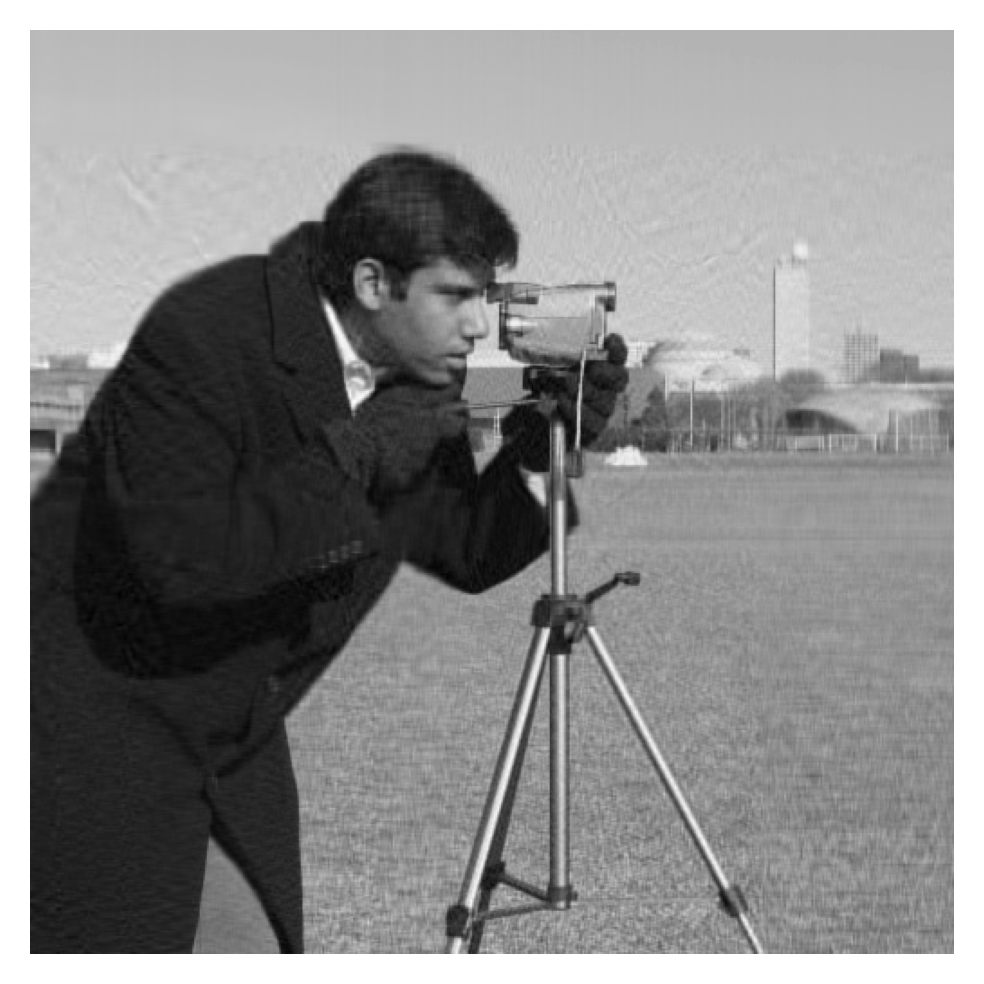
\includegraphics[width=.15\textwidth]{camera_svd_71_estimate}%
  \hfill
  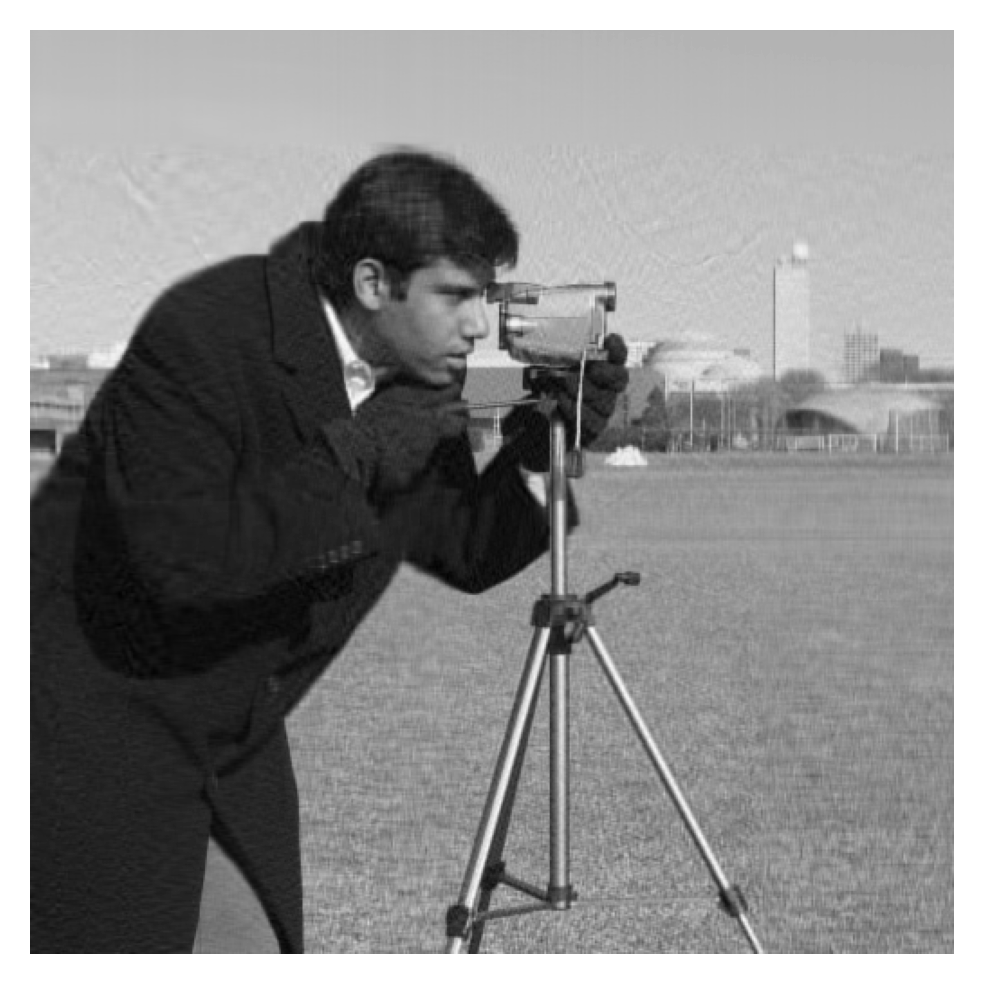
\includegraphics[width=.15\textwidth]{camera_svd_76_estimate}%
  \hfill
  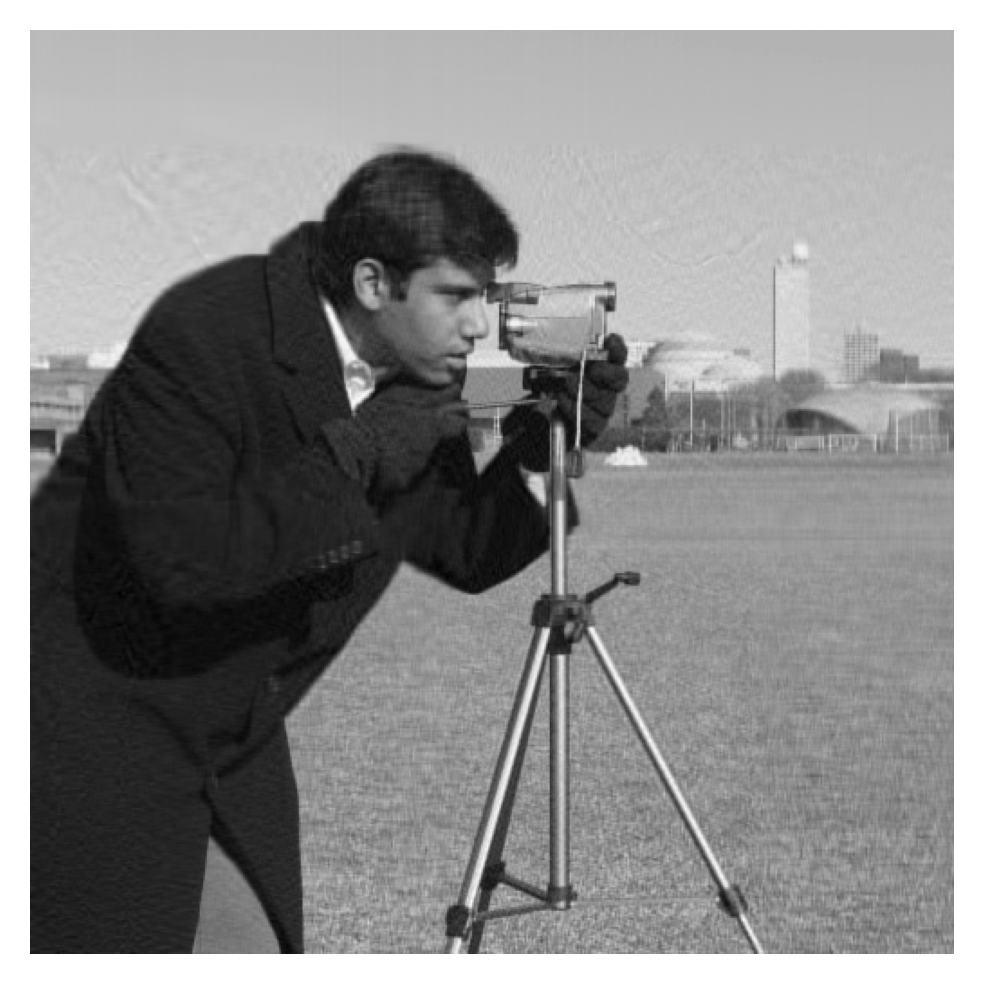
\includegraphics[width=.15\textwidth]{camera_svd_81_estimate}%
  \hfill
  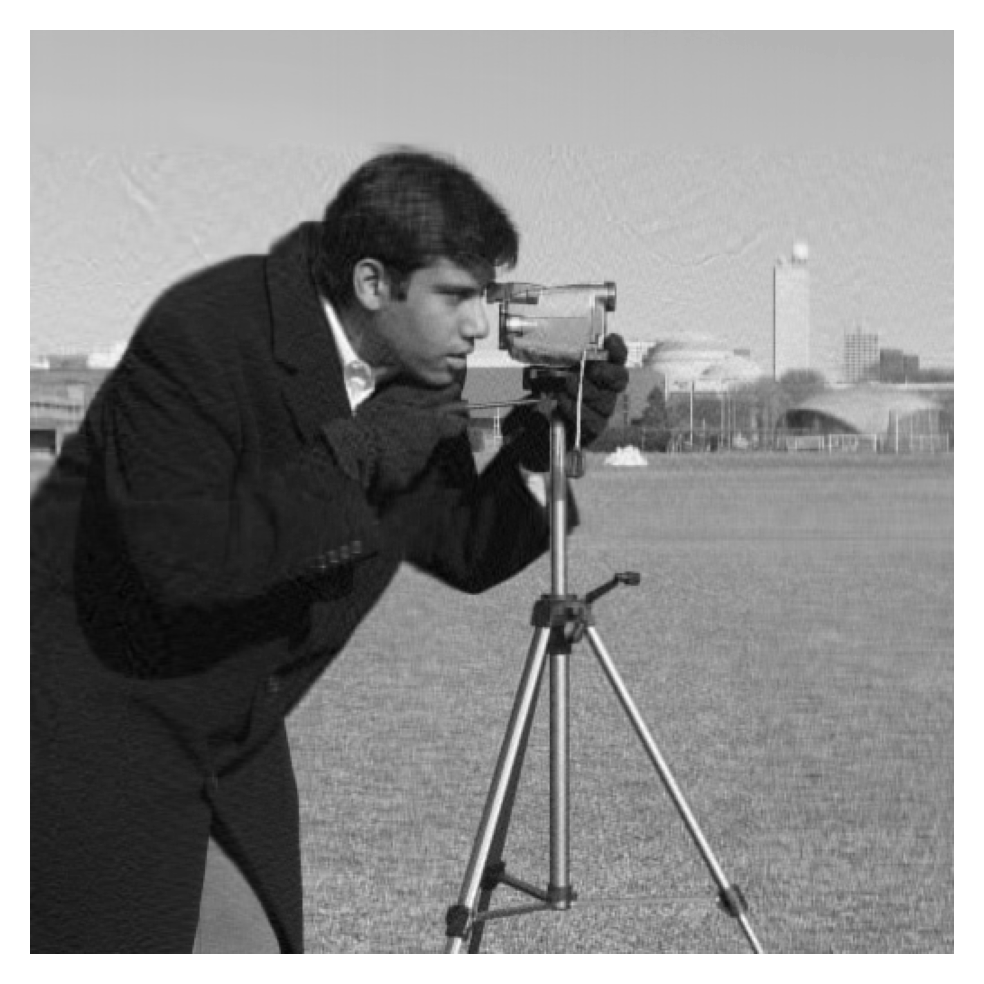
\includegraphics[width=.15\textwidth]{camera_svd_86_estimate}

  \vfill
\end{frame}

\section{Extracting coherent patterns}
\begin{frame}
  \sectionpage
\end{frame}

\begin{frame}
  Add Yale B faces
\end{frame}

\begin{frame}
  Add video of the cavity
\end{frame}


{
  \setbeamercolor*{background canvas}{bg=white}

\begin{frame}%{A gallery of fluid motion}
  \vfill
  \centering

  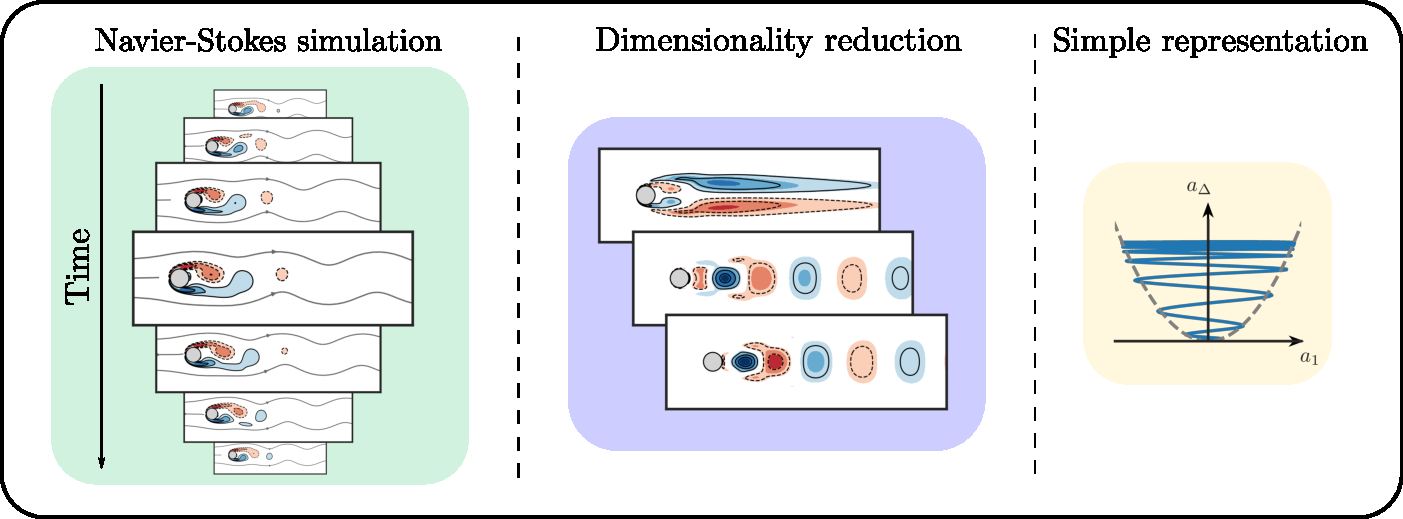
\includegraphics[width=\textwidth]{reduced_order_modeling}
  \vfill
\end{frame}

}

\begin{frame}%{Encoder-Decoder network}
  \centering

  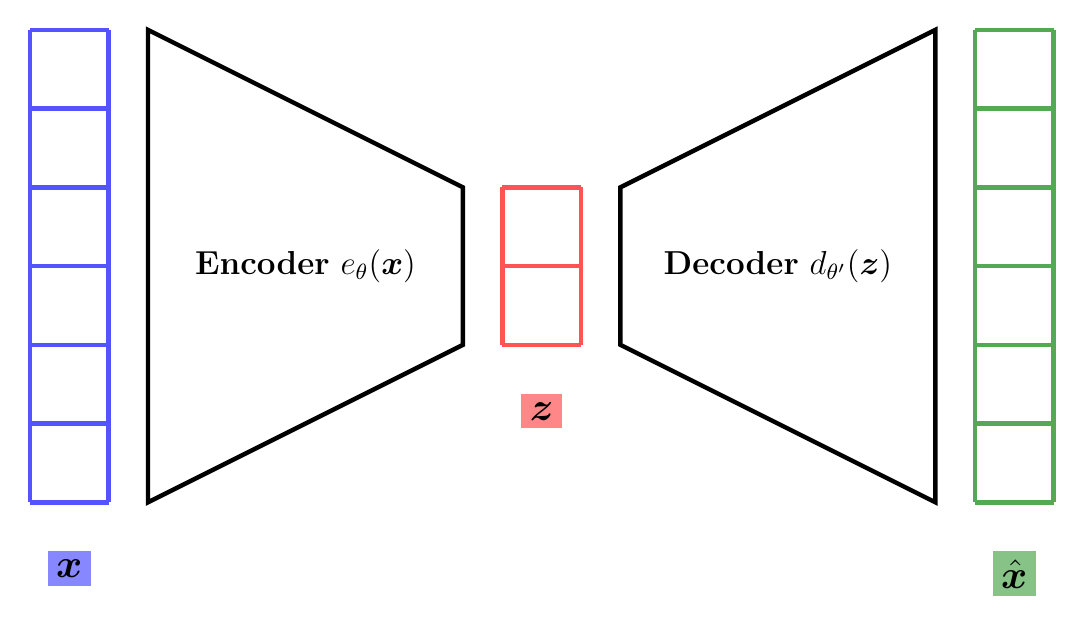
\begin{tikzpicture}
    % \draw[help lines, step=1] (-7, -4) grid (6, 4);

    \draw[step=1, ultra thick, draw=blue!67] (-7, -3) grid (-6, 3);

    \draw[step=1, ultra thick, draw=Green!67] (5, -3) grid (6, 3);

    \draw[step=1, ultra thick, draw=red!67] (-1, -1) grid (0, 1);

    \draw[ultra thick] (-5.5, -3) -- (-1.5, -1) -- (-1.5, 1) -- (-5.5, 3) -- cycle;

    \draw[ultra thick] (4.5, -3) -- (0.5, -1) -- (0.5, 1) -- (4.5, 3) -- cycle;

    \node[anchor=north] at (-6.5, -3.5) {\highlightdark{blue}{\Large $\bm{x}$}};
    \node[anchor=north] at (-0.5, -1.5) {\highlightdark{red}{\Large $\bm{z}$}};
    \node[anchor=north] at (5.5, -3.5) {\highlightdark{Green}{\Large $\hat{\bm{x}}$}};

    \node[] at (-3.5, 0) {\large \textbf{Encoder} $e_{\theta}(\bm{x})$};
    \node[] at (2.5, 0) {\large \textbf{Decoder} $d_{\theta^{\prime}}(\bm{z})$};

  \end{tikzpicture}

  \vspace{-1.5cm}
\end{frame}

\begin{frame}
  \vfill
  {
  \Large
  \[
    \min_{\theta, \theta^{\prime}} \ \sum_{i=1}^N \| \tikzmarknode{a} {\highlightdark{blue}{$\bm{x}_i$}} - \tikzmarknode{c} {\highlightdark{Green}{$( d_{\theta^{\prime}} \circ$ {\highlightdark{red}{$e_{\theta} )(\bm{x}_i)$}}}} \|_2^2
  \]
  }
  \begin{tikzpicture}[overlay, remember picture, >=stealth, nodes={align=left, inner ysep=1pt}, <-]

    \path (a.south) ++ (0, -2em) node[anchor=north east, color=blue!67] (data){Ground truth};
    \draw [color=blue!87] (a.south) |- ([xshift=-0.3ex, color=blue] data.south west);

    \path (c.north) ++ (0, 2em) node[anchor=south west, color=Green!67] (estimate){Estimate};
    \draw [color=Green!87] (c.north) |- ([xshift=0.3ex, color=Green] estimate.south east);

  \end{tikzpicture}

  \vfill
\end{frame}

\begin{frame}
  \vfill

  \begin{overprint}
    \onslide<1>
    \Large
    \[
    \begin{aligned}
      \minimize_{\bm{P}, \bm{Q}} & \quad \sum_{i=1}^N \| \bm{x}_i - \bm{PQ}^T \bm{x}_i \|_2^2 \\
      \subto & \quad \mathrm{rank~} \bm{P} = \mathrm{rank~} \bm{Q} = r
    \end{aligned}
    \]

    \onslide<2>
    \Large
    \[
    \begin{aligned}
      \minimize_{\bm{P}} & \quad \sum_{i=1}^N \| \bm{x}_i - \bm{PP}^T \bm{x}_i \|_2^2 \\
      \subto & \quad \mathrm{rank~} \bm{P} = r
    \end{aligned}
    \]

  \end{overprint}

  \vfill
\end{frame}

\begin{frame}
  \vfill
  \Large
  \[
  \begin{aligned}
    \minimize_{\bm{P}} & \quad \| \bm{X} - \bm{PP}^T \bm{X} \|_F^2 \\
    \subto & \quad \bm{P}^T \bm{P} = \bm{I}_r
  \end{aligned}
  \]

  \vfill
\end{frame}

\begin{frame}
  \vfill

  \begin{tcolorbox}[
    enhanced,
    coltitle=black,
    coltext=white,
    colback=black,
    title=\textbf{Proper Orthogonal Decomposition},
    frame style tile={width=\paperwidth}{background.jpg}
    ]

    \medskip

    \large

    \[
    \bm{P} \boldsymbol{\Lambda} = \bm{C}_{\bm{xx}} \bm{P}
    \]

    \medskip
  \end{tcolorbox}

  \vfill

  $\bm{P}$ corresponds to the left singular vectors of $\bm{X}$.
  The latent representation is given by $\bm{z}_i = \bm{P}^T \bm{x}_i$.
  The optimal rank of the model can be inferred from the distribution of the PCA eigenvalues $\boldsymbol{\Lambda} = \boldsymbol{\Sigma}^2$.

  \vfill
\end{frame}

\begin{frame}{Eigenfaces}

\end{frame}

\begin{frame}{Shear-driven cavity POD modes}
  Add POD modes
\end{frame}

\begin{frame}{Shear-driven cavity POD modes}
  Add phase portraits
\end{frame}

{
\setbeamercolor*{background canvas}{bg=white}

\begin{frame}
  \textcolor{black}{Add cylinder flow and pressure coefficient}
\end{frame}

}

\begin{frame}%{Encoder-Decoder network}
  \centering

  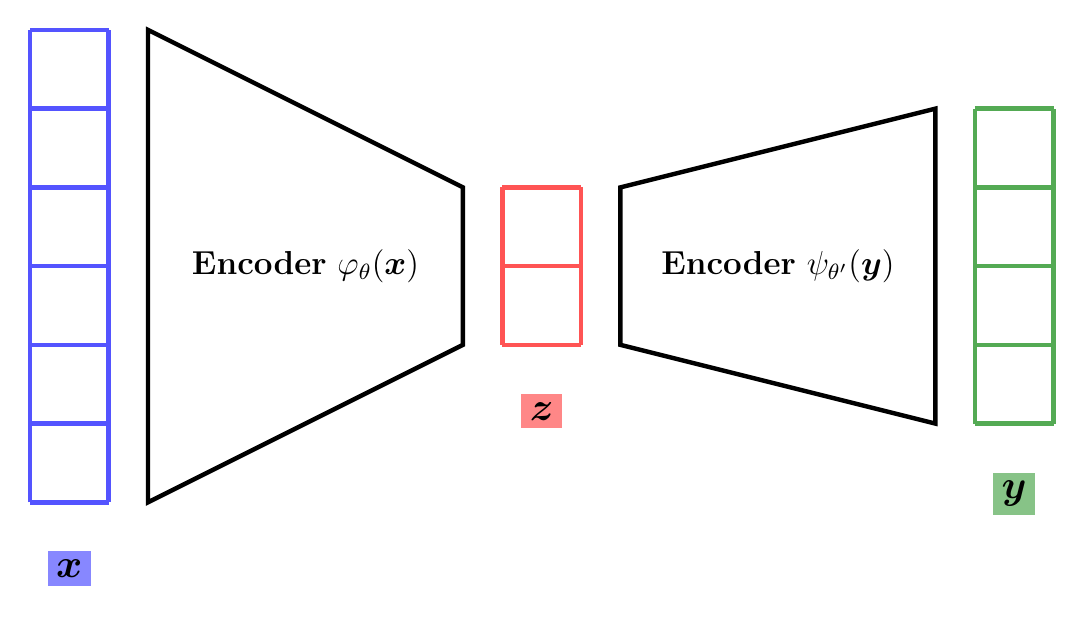
\begin{tikzpicture}
    % \draw[help lines, step=1] (-7, -4) grid (6, 4);

    \draw[step=1, ultra thick, draw=blue!67] (-7, -3) grid (-6, 3);

    \draw[step=1, ultra thick, draw=Green!67] (5, -2) grid (6, 2);

    \draw[step=1, ultra thick, draw=red!67] (-1, -1) grid (0, 1);

    \draw[ultra thick] (-5.5, -3) -- (-1.5, -1) -- (-1.5, 1) -- (-5.5, 3) -- cycle;

    \draw[ultra thick] (4.5, -2) -- (0.5, -1) -- (0.5, 1) -- (4.5, 2) -- cycle;

    \node[anchor=north] at (-6.5, -3.5) {\highlightdark{blue}{\Large $\bm{x}$}};
    \node[anchor=north] at (-0.5, -1.5) {\highlightdark{red}{\Large $\bm{z}$}};
    \node[anchor=north] at (5.5, -2.5) {\highlightdark{Green}{\Large $\bm{y}$}};

    \node[] at (-3.5, 0) {\large \textbf{Encoder} $\varphi_{\theta}(\bm{x})$};
    \node[] at (2.5, 0) {\large \textbf{Encoder} $\psi_{\theta^{\prime}}(\bm{y})$};

  \end{tikzpicture}

  \vspace{-1.5cm}
\end{frame}

\begin{frame}
  \vfill

  \Large
  \[
  \min_{\theta, \theta^{\prime}} \quad \sum_{i=1}^N \| \varphi_{\theta}(\bm{x}_i) - \psi_{\theta^{\prime}}(\bm{y}_i) \|_2^2
  \]

  \vfill
\end{frame}

\begin{frame}
  \vfill
  \Large

  \[
  \begin{aligned}
    \minimize_{\bm{P}, \bm{Q}} & \quad \sum_{i=1}^N \| \bm{P}^T \bm{y}_i - \bm{Q}^T \bm{x}_i \|_2^2 \\
    \subto & \quad \mathrm{rank~} \bm{P} = \mathrm{rank~} \bm{Q} = r
  \end{aligned}
  \]
  \vfill
\end{frame}

\begin{frame}
  \vfill
  \Large
  \[
  \begin{aligned}
    \minimize_{\bm{P}, \bm{Q}} & \quad \| \bm{P}^T \bm{Y} - \bm{Q}^T \bm{X} \|_F^2 \\
    \subto & \quad \bm{P}^T \bm{C}_{yy} \bm{P} = \bm{Q}^T \bm{C}_{xx} \bm{Q} = \bm{I}_r
  \end{aligned}
  \]
  \vfill
\end{frame}

\begin{frame}

  \vfill

    \begin{tcolorbox}[
      enhanced,
      coltitle=black,
      coltext=white,
      colback=black,
      title=\textbf{Canonical Correlation Analysis},
      frame style tile={width=\paperwidth}{background.jpg}
      ]

      \medskip

      \Large

      \[
      \begin{bmatrix}
        \bm{C}_{yy} & \bm{0} \\
        \bm{0} & \bm{C}_{xx}
      \end{bmatrix}
      \begin{bmatrix}
        \bm{P} \\ \bm{Q}
      \end{bmatrix}
      \boldsymbol{\Sigma}
      =
      \begin{bmatrix}
        \bm{0} & \bm{C}_{yx} \\
        \bm{C}_{xy} & \bm{0}
      \end{bmatrix}
      \begin{bmatrix}
        \bm{P} \\ \bm{Q}
      \end{bmatrix}
      \]

      \medskip
    \end{tcolorbox}

    \vfill

    CCA relies on a \emph{generalized eigenproblem}.
    $\bm{P}$ and $\bm{Q}$ describe the encoders such that the latent representations $\bm{z} = \bm{Q}^T \bm{x}$ and $\bm{z}^{\prime} = \bm{P}^T \bm{Y}$ are as similar as possible.
    It is closely related to the concept of \emph{mutual information}.

    \vfill
\end{frame}

{
\setbeamercolor*{background canvas}{bg=white}

\begin{frame}
  \textcolor{black}{Add cylinder flow and pressure coefficient}
\end{frame}

}

\section{Optimal sensor placement}
\begin{frame}
  \sectionpage
\end{frame}

\begin{frame}

\end{frame}

\begin{frame}
  \vfill

  {
  \Large
  \[
  \tikzmarknode{a} {\highlightdark{blue}{$\bm{y}$}}
  =
  \tikzmarknode{b} {\highlightdark{red}{$\bm{C}$}}
  \tikzmarknode{c} {\highlightdark{Green}{$\bm{x}$}}
  \]
  }

  \begin{tikzpicture}[overlay, remember picture, >=stealth, nodes={align=left, inner ysep=1pt}, <-]

    \path (a.south) ++ (0, -2em) node[anchor=north east, color=blue!67] (data){Observations};
    \draw [color=blue!87] (a.south) |- ([xshift=-0.3ex, color=blue] data.south west);

    \path (b.north) ++ (0, 2em) node[anchor=south west, color=red!67] (obs){Measurement operator};
    \draw [color=red!87] (b.north) |- ([xshift=0.3ex, color=red] obs.south east);

    \path (c.north) ++ (0, -2em) node[anchor=north west, color=Green!67] (estimate){Full state};
    \draw [color=Green!87] (c.south) |- ([xshift=-0.3ex, color=Green] estimate.south east);

  \end{tikzpicture}

  \vfill
\end{frame}

{
\setbeamercolor*{background canvas}{bg=white}

\begin{frame}
  \vfill
  \centering

  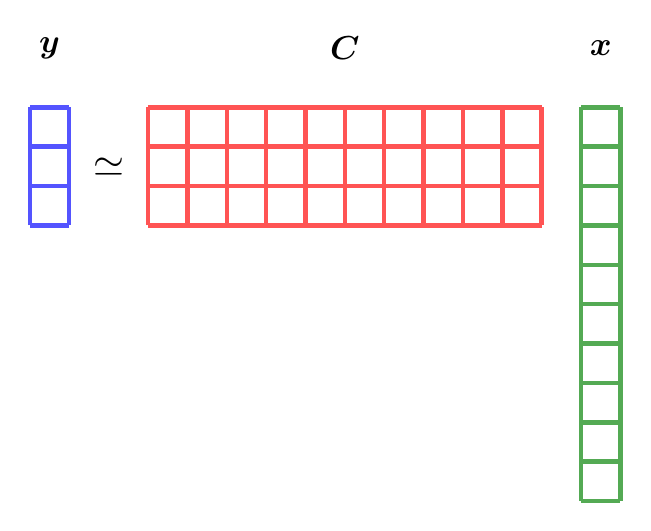
\begin{tikzpicture}
    %\draw[help lines, step=1] (-7, -4) grid (6, 4);

    \draw[step=0.5, ultra thick, draw=blue!67] (-7, -1) grid (-6.5, 0.5);

    \node[anchor=south] at (-6, -0.5) {\Large \textcolor{black}{$\simeq$}};

    \draw[step=0.5, ultra thick, draw=red!67] (-5.5, -1) grid (-0.5, 0.5);

    \draw[step=0.5, ultra thick, draw=Green!67] (0, 0.5) grid (0.5, -4.5);

    \node[text centered] at (-6.75, 1.25) {\large \textcolor{black}{$\bm{y}$}};
    \node[text centered] at (-3, 1.25) {\large \textcolor{black}{$\bm{C}$}};
    \node[text centered] at (0.25, 1.25) {\large \textcolor{black}{$\bm{x}$}};

    % \draw[draw=red, fill=black, ultra thick] (-5.5, -1) rectangle (-5, -0.5);
    % \draw[draw=red, fill=black, ultra thick] (-1.5, -.5) rectangle (-1, 0);
    % \draw[draw=red, fill=black, ultra thick] (-3.5, 0) rectangle (-3, 0.5);

  \end{tikzpicture}

  \vfill
\end{frame}

\begin{frame}
  \vfill
  \centering

  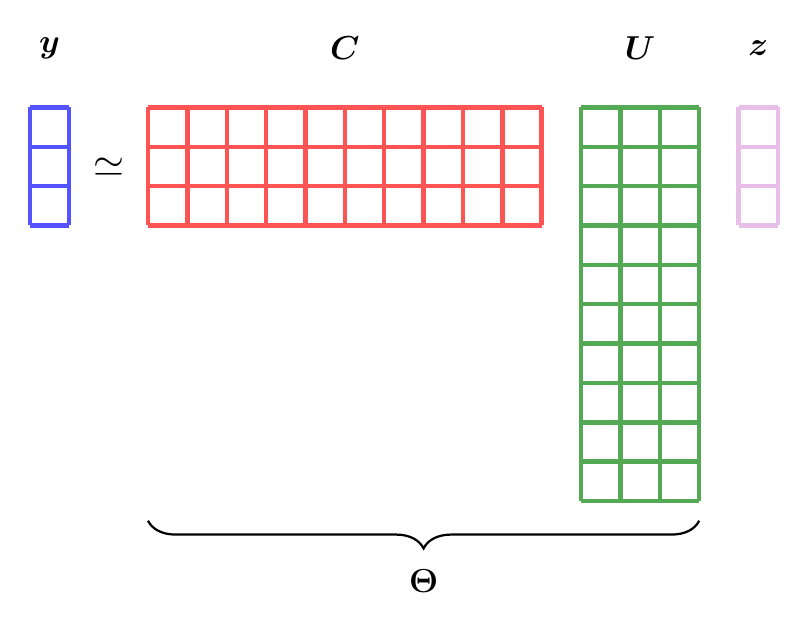
\begin{tikzpicture}
    %\draw[help lines, step=1] (-7, -4) grid (6, 4);

    \draw[step=0.5, ultra thick, draw=blue!67] (-7, -1) grid (-6.5, 0.5);

    \node[anchor=south] at (-6, -0.5) {\Large \textcolor{black}{$\simeq$}};

    \draw[step=0.5, ultra thick, draw=red!67] (-5.5, -1) grid (-0.5, 0.5);

    \draw[step=0.5, ultra thick, draw=Green!67] (0, 0.5) grid (1.5, -4.5);

    \draw[step=0.5, ultra thick, draw=Plum!67] (2, -1) grid (2.5, 0.5);
    \draw[ultra thick, Plum!67] (2, 0.5) -- (2, -1);

    \node[text centered] at (-6.75, 1.25) {\large \textcolor{black}{$\bm{y}$}};
    \node[text centered] at (-3, 1.25) {\large \textcolor{black}{$\bm{C}$}};
    \node[text centered] at (0.75, 1.25) {\large \textcolor{black}{$\bm{U}$}};
    \node[text centered] at (2.25, 1.25) {\large \textcolor{black}{$\bm{z}$}};

    % \draw[draw=red, fill=black, ultra thick] (-5.5, -1) rectangle (-5, -0.5);
    % \draw[draw=red, fill=black, ultra thick] (-1.5, -.5) rectangle (-1, 0);
    % \draw[draw=red, fill=black, ultra thick] (-3.5, 0) rectangle (-3, 0.5);

    \draw [decorate, thick, black, decoration={brace, mirror, amplitude=10pt}] (-5.5, -4.75) -- (1.5, -4.75);
    \node [black, below] at (-2, -5.25) {\large $\boldsymbol{\Theta}$};
  \end{tikzpicture}

  \vfill
\end{frame}

\begin{frame}
  \vfill
  \centering

  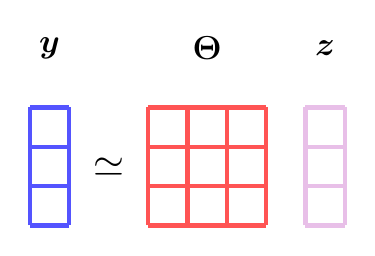
\begin{tikzpicture}
    %\draw[help lines, step=1] (-7, -4) grid (6, 4);

    \draw[step=0.5, ultra thick, draw=blue!67] (-7, -1) grid (-6.5, 0.5);

    \node[anchor=south] at (-6, -0.5) {\Large \textcolor{black}{$\simeq$}};

    \draw[step=0.5, ultra thick, draw=red!67] (-5.5, -1) grid (-4, 0.5);

    \draw[step=0.5, ultra thick, draw=Plum!67] (-3.5, -1) grid (-3, 0.5);
    % \draw[ultra thick, Plum!67] (2, 0.5) -- (2, -1);

    \node[text centered] at (-6.75, 1.25) {\large \textcolor{black}{$\bm{y}$}};
    \node[text centered] at (-4.75, 1.25) {\large \textcolor{black}{$\boldsymbol{\Theta}$}};
    \node[text centered] at (-3.25, 1.25) {\large \textcolor{black}{$\bm{z}$}};

  \end{tikzpicture}

  \vfill
\end{frame}

}

\begin{frame}
  \vfill

  \Large

  \[
  \minimize_{\bm{z}} \quad \| \bm{y}  - \boldsymbol{\Theta} \bm{z} \|_2
  \]

  \vfill
\end{frame}


\begin{frame}
  \vfill

  \Large

  \[
  \bm{z} = \boldsymbol{\Theta}^{-1} \bm{y}
  \]

  \vfill
\end{frame}

\begin{frame}
  \vfill

  \Large
  \[
  \maximize_{\bm{C}} \quad \vert \det(\bm{CU}) \vert
  \]

  \vfill
\end{frame}


\begin{frame}
  \vfill

  \Large
  \[
  \begin{aligned}
    \maximize_{\bm{C}} \quad & \vert \det(\bm{CU}) \vert \\
    \subto \quad & \bm{C}_i \in \left\{ \bm{e}_j \right\}_{j=1, n}
  \end{aligned}
  \]

  \vfill
\end{frame}

\begin{frame}
  QR sensor placement algorithm
\end{frame}

\begin{frame}{Extended Yale B Face dataset}

\end{frame}

\begin{frame}{Shear-driven cavity flow}

\end{frame}

\section{State estimation and low-rank sensing}
\begin{frame}
  \sectionpage
\end{frame}


\begin{frame}
  \vfill

  {
  \Large
  \[
  \tikzmarknode{a} {\highlightdark{blue}{$\bm{y}$}}
  =
  \tikzmarknode{b} {\highlightdark{red}{$\bm{C}$}}
  \tikzmarknode{c} {\highlightdark{Green}{$\bm{x}$}}
  \]
  }

  \begin{tikzpicture}[overlay, remember picture, >=stealth, nodes={align=left, inner ysep=1pt}, <-]

    \path (a.south) ++ (0, -2em) node[anchor=north east, color=blue!67] (data){Observations};
    \draw [color=blue!87] (a.south) |- ([xshift=-0.3ex, color=blue] data.south west);

    \path (b.north) ++ (0, 2em) node[anchor=south west, color=red!67] (obs){Measurement operator};
    \draw [color=red!87] (b.north) |- ([xshift=0.3ex, color=red] obs.south east);

    \path (c.north) ++ (0, -2em) node[anchor=north west, color=Green!67] (estimate){Full state};
    \draw [color=Green!87] (c.south) |- ([xshift=-0.3ex, color=Green] estimate.south east);

  \end{tikzpicture}

  \vfill
\end{frame}

{
\setbeamercolor*{background canvas}{bg=white}

\begin{frame}
  \vfill
  \centering

  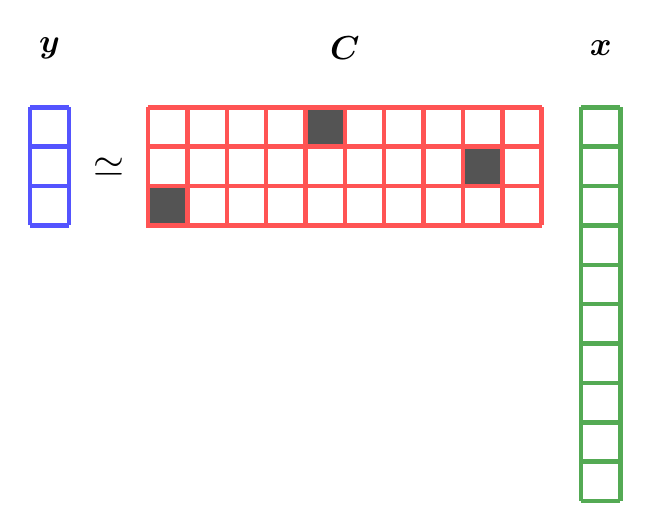
\begin{tikzpicture}
    %\draw[help lines, step=1] (-7, -4) grid (6, 4);

    \draw[step=0.5, ultra thick, draw=blue!67] (-7, -1) grid (-6.5, 0.5);

    \node[anchor=south] at (-6, -0.5) {\Large \textcolor{black}{$\simeq$}};

    \draw[step=0.5, ultra thick, draw=red!67] (-5.5, -1) grid (-0.5, 0.5);

    \draw[step=0.5, ultra thick, draw=Green!67] (0, 0.5) grid (0.5, -4.5);

    \node[text centered] at (-6.75, 1.25) {\large \textcolor{black}{$\bm{y}$}};
    \node[text centered] at (-3, 1.25) {\large \textcolor{black}{$\bm{C}$}};
    \node[text centered] at (0.25, 1.25) {\large \textcolor{black}{$\bm{x}$}};

    \draw[draw=red!67, fill=black!67, ultra thick] (-5.5, -1) rectangle (-5, -0.5);
    \draw[draw=red!67, fill=black!67, ultra thick] (-1.5, -.5) rectangle (-1, 0);
    \draw[draw=red!67, fill=black!67, ultra thick] (-3.5, 0) rectangle (-3, 0.5);

  \end{tikzpicture}

  \vfill
\end{frame}

\begin{frame}
  \vfill
  \centering

  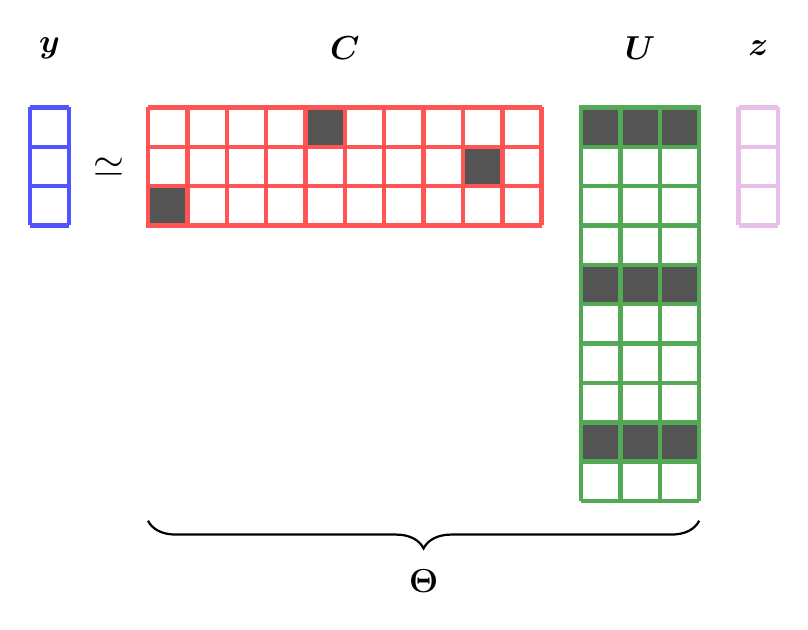
\begin{tikzpicture}
    % \draw[help lines, step=1, black] (-7, -4) grid (6, 4);

    \draw[step=0.5, ultra thick, draw=blue!67] (-7, -1) grid (-6.5, 0.5);

    \node[anchor=south] at (-6, -0.5) {\Large \textcolor{black}{$\simeq$}};

    \draw[step=0.5, ultra thick, draw=red!67] (-5.5, -1) grid (-0.5, 0.5);

    \draw[step=0.5, ultra thick, draw=Green!67] (0, 0.5) grid (1.5, -4.5);

    \draw[step=0.5, ultra thick, draw=Plum!67] (2, 0.5) grid (2.5, -1);
    \draw[ultra thick, Plum!67] (2, 0.5) -- (2, -1);

    \node[text centered] at (-6.75, 1.25) {\large \textcolor{black}{$\bm{y}$}};
    \node[text centered] at (-3, 1.25) {\large \textcolor{black}{$\bm{C}$}};
    \node[text centered] at (0.75, 1.25) {\large \textcolor{black}{$\bm{U}$}};
    \node[text centered] at (2.25, 1.25) {\large \textcolor{black}{$\bm{z}$}};

    \draw[draw=red!67, fill=black!67, ultra thick] (-5.5, -1) rectangle (-5, -0.5);
    \draw[draw=red!67, fill=black!67, ultra thick] (-1.5, -.5) rectangle (-1, 0);
    \draw[draw=red!67, fill=black!67, ultra thick] (-3.5, 0) rectangle (-3, 0.5);

    \draw[draw=Green!67, fill=black!67, ultra thick] (0, 0.5) rectangle (0.5, 0);
    \draw[draw=Green!67, fill=black!67, ultra thick] (0.5, 0.5) rectangle (1, 0);
    \draw[draw=Green!67, fill=black!67, ultra thick] (1, 0.5) rectangle (1.5, 0);

    \draw[draw=Green!67, fill=black!67, ultra thick] (0, -1.5) rectangle (0.5, -2);
    \draw[draw=Green!67, fill=black!67, ultra thick] (0.5, -1.5) rectangle (1, -2);
    \draw[draw=Green!67, fill=black!67, ultra thick] (1, -1.5) rectangle (1.5, -2);

    \draw[draw=Green!67, fill=black!67, ultra thick] (0, -3.5) rectangle (0.5, -4);
    \draw[draw=Green!67, fill=black!67, ultra thick] (0.5, -3.5) rectangle (1, -4);
    \draw[draw=Green!67, fill=black!67, ultra thick] (1, -3.5) rectangle (1.5, -4);


    \draw [decorate, thick, black, decoration={brace, mirror, amplitude=10pt}] (-5.5, -4.75) -- (1.5, -4.75);
    \node [black, below] at (-2, -5.25) {\large $\boldsymbol{\Theta}$};
  \end{tikzpicture}

  \vfill
\end{frame}


\begin{frame}
  \vfill
  \centering

  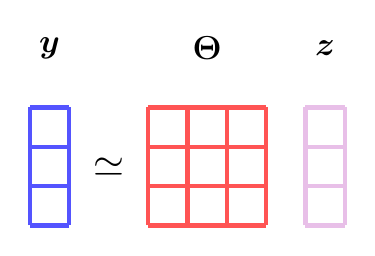
\begin{tikzpicture}
    %\draw[help lines, step=1] (-7, -4) grid (6, 4);

    \draw[step=0.5, ultra thick, draw=blue!67] (-7, -1) grid (-6.5, 0.5);

    \node[anchor=south] at (-6, -0.5) {\Large \textcolor{black}{$\simeq$}};

    \draw[step=0.5, ultra thick, draw=red!67] (-5.5, -1) grid (-4, 0.5);

    \draw[step=0.5, ultra thick, draw=Plum!67] (-3.5, -1) grid (-3, 0.5);
    % \draw[ultra thick, Plum!67] (2, 0.5) -- (2, -1);

    \node[text centered] at (-6.75, 1.25) {\large \textcolor{black}{$\bm{y}$}};
    \node[text centered] at (-4.75, 1.25) {\large \textcolor{black}{$\boldsymbol{\Theta}$}};
    \node[text centered] at (-3.25, 1.25) {\large \textcolor{black}{$\bm{z}$}};

  \end{tikzpicture}

  \vfill
\end{frame}

}

\begin{frame}
  \vfill
  \begin{minipage}{.48\textwidth}
    \centering
    \underline{\textbf{Undertermined problem}}
  \end{minipage}%
  \hfill
  \begin{minipage}{.48\textwidth}
    \centering
    \underline{\textbf{Overdetermined problem}}
  \end{minipage}

  \bigskip

  \begin{minipage}{.48\textwidth}
    \large
    \[
    \begin{aligned}
      \minimize_{\bm{z}} & \quad \| \bm{z} \|_2 \\
      \subto & \quad \bm{y} = \boldsymbol{\Theta} \bm{z}
    \end{aligned}
    \]
  \end{minipage}%
  \hfill
  \begin{minipage}{.48\textwidth}
    \large
    \[
    \minimize_{\bm{z}} \quad \| \bm{y} - \boldsymbol{\Theta} \bm{z} \|_2^2
    \]
  \end{minipage}

  \vfill
\end{frame}

\begin{frame}
  \vfill
  \centering
  \underline{\textbf{Regularized problem}}

  %\bigskip

  \large
  \[
  \minimize_{\bm{z}} \quad \| \bm{y} - \boldsymbol{\Theta} \bm{z} \|_2^2 + \lambda \| \bm{z} \|_2^2
  \]
  \vfill
\end{frame}

\begin{frame}
  \vfill
  \centering
  \underline{\textbf{Regularized and constrained problem}}

  %\bigskip

  \large
  \[
  \begin{aligned}
    \minimize_{\bm{z}} & \quad \| \bm{y} - \boldsymbol{\Theta} \bm{z} \|_2^2 + \lambda \| \bm{z} \|_2^2 \\
    \subto & \quad \vert z_i \vert \leq 2 \sigma_i \quad \forall \ i
  \end{aligned}
  \]
  \vfill
\end{frame}

{
\setbeamercolor*{background canvas}{bg=white}

\begin{frame}
  \textcolor{black}{Add figures from SIAM paper}
\end{frame}
}


\section{Reduced-order modeling}
\begin{frame}
  \sectionpage
\end{frame}

\begin{frame}

\end{frame}


\begin{frame}
  \vfill

  {
  \Large
  \[
  \begin{aligned}
    \dfrac{\mathrm{d} \bm{x}}{\mathrm{d}t} & = \tikzmarknode{a} {\highlightdark{red}{$\bm{A}$}} \bm{x} + \tikzmarknode{b} {\highlightdark{blue}{$\bm{B}$}} \bm{u} \\
    \bm{y} & = \tikzmarknode{c} {\highlightdark{Green}{$\bm{C}$}} \bm{x} + \tikzmarknode{d} {\highlightdark{Plum}{$\bm{D}$}} \bm{u}
  \end{aligned}
  \]
  }

  \begin{tikzpicture}[overlay, remember picture, >=stealth, nodes={align=left, inner ysep=1pt}, <-]

    \path (a.north) ++ (0, 2em) node[anchor=south east, color=red!67] (dynamics){Natural dynamics};
    \draw [color=red!87] (a.north) |- ([xshift=0.3ex, color=blue] dynamics.south west);

    \path (b.north) ++ (0, 2em) node[anchor=south west, color=blue!67] (actuators){Actuators};
    \draw [color=blue!87] (b.north) |- ([xshift=0.3ex, color=blue] actuators.south east);

    \path (c.south) ++ (0, -2em) node[anchor=north east, color=Green!67] (obs){Measurements};
    \draw [color=Green!87] (c.south) |- ([xshift=-0.3ex, color=Green] obs.south west);

    \path (d.south) ++ (0, -2em) node[anchor=north west, color=Plum!67] (feed){Feedthrough};
    \draw [color=Plum!87] (d.south) |- ([xshift=-0.3ex, color=Plum] feed.south east);

  \end{tikzpicture}

  \vfill
\end{frame}

\begin{frame}
  \vfill
  \centering

  \underline{\textbf{Controlability Gramian}}

  \Large
  {
    \[
    \bm{W}_{\mathcal{C}} = \displaystyle \int_0^{\infty} e^{\tau \bm{A}} \bm{BB}^* e^{\tau \bm{A}^*} \ \mathrm{d}\tau
    \]
  }

  \vfill
\end{frame}

\begin{frame}
  \vfill
  \centering

  \underline{\textbf{Observability Gramian}}

  \Large
  {
    \[
    \bm{W}_{\mathcal{O}} = \displaystyle \int_0^{\infty} e^{\tau \bm{A}^*} \bm{C}^* \bm{C} e^{\tau \bm{A}} \ \mathrm{d}\tau
    \]
  }

  \vfill
\end{frame}


\begin{frame}
  \vfill

  \begin{tcolorbox}[
    enhanced,
    coltitle=black,
    coltext=white,
    colback=black,
    title=\textbf{Balancing transform / Balanced tuncation},
    frame style tile={width=\paperwidth}{background.jpg}
    ]

    \medskip
    \Large

    \[
    \begin{bmatrix}
      \bm{0} & \bm{I} \\
      \bm{I} & \bm{0}
    \end{bmatrix}
    \begin{bmatrix}
      \bm{P} \\ \bm{Q}
    \end{bmatrix}
    \boldsymbol{\Sigma}
      =
    \begin{bmatrix}
      \bm{W}_{\mathcal{O}} & \bm{0} \\
      \bm{0} & \bm{W}_{\mathcal{C}}
    \end{bmatrix}
    \begin{bmatrix}
      \bm{P} \\ \bm{Q}
    \end{bmatrix}
    \]

    \medskip
  \end{tcolorbox}

  \vfill

  BT discards modes which are highly controlable but poorly observable, and vice versa.
  The transformed system is \textbf{balanced}.
  Its Gramians are given by $\hat{\bm{W}}_{\mathcal{O}} = \hat{\bm{W}}_{\mathcal{C}} = \boldsymbol{\Sigma}$ where $\boldsymbol{\Sigma}$ are the \emph{Hankel singular values} of the system.

  \vfill
\end{frame}

\begin{frame}
  \vfill

  \centering
  \underline{\textbf{Balanced Proper Orthogonal Decomposition}}

  \vfill
  \begin{overprint}
    \onslide<1>
    \begin{enumerate}
      \item[1.] For each actuator, compute the corresponding impulse reponse
      %
      \[
      \bm{X}_i
      =
      \begin{bmatrix}
        \bm{B}_i & e^{\Delta t \bm{A}} \bm{B}_i & e^{2\Delta t \bm{A}} \bm{B}_i & \cdots & e^{n \Delta t \bm{A}} \bm{B}_i
      \end{bmatrix}
      \]
      %
      and assemble the data matrix $\bm{X} = \begin{bmatrix} \bm{X}_1 & \bm{X}_2 & \cdots & \bm{X}_p \end{bmatrix}$.
    \end{enumerate}

    \onslide<2>
    \begin{enumerate}
      \item[2.] For each sensor, compute the corresponding \textbf{adjoint} impulse reponse
      %
      \[
      \bm{Y}_i
      =
      \begin{bmatrix}
        \bm{C}^*_i & e^{\Delta t \bm{A}^*} \bm{C}^*_i & e^{2\Delta t \bm{A}^*} \bm{C}^*_i & \cdots & e^{n \Delta t \bm{A}^*} \bm{C}_i^*
      \end{bmatrix}
      \]
      %
      and assemble the data matrix $\bm{Y} = \begin{bmatrix} \bm{Y}_1 & \bm{Y}_2 & \cdots & \bm{Y}_q \end{bmatrix}$.
    \end{enumerate}

    \onslide<3>
    \begin{enumerate}
      \item[3.] Compute the SVD of $\bm{Y}^T \bm{X}$
      %
      \[
      \bm{Y}^T \bm{X} = \bm{U} \boldsymbol{\Sigma} \bm{V}^T
      \]
      %
      where $\boldsymbol{\Sigma}$ are the \emph{Hankel singular values} of the system.
    \end{enumerate}

    \onslide<4>
    \begin{enumerate}
      \item[4.] Compute the first $r$ columns and rows of the balancing transform as
      %
      \[
      \bm{P} = \bm{X} \bm{V} \boldsymbol{\Sigma}^{-\frac12} \quad \text{and} \quad \bm{Q} = \bm{Y} \bm{U} \boldsymbol{\Sigma}^{-\frac12}
      \]
      %
      and proceed with the construction of the reduced-order model.
    \end{enumerate}

  \end{overprint}

  \vfill
\end{frame}

\begin{frame}
  \vfill

  \centering
  \underline{\textbf{Petrov-Galerkin projection}}

  \bigskip

  \begin{overprint}
    \onslide<1>
    \Large
    \[
    \begin{aligned}
      \dfrac{\mathrm{d} \hat{\bm{x}}}{\mathrm{d}t} & = \hat{\bm{A}} \hat{\bm{x}} + \hat{\bm{B}} \bm{u} \\
      \hat{\bm{y}} & = \hat{\bm{C}} \hat{\bm{x}} + \hat{\bm{D}} \bm{u}
    \end{aligned}
    \]

    \onslide<2>
    \Large
    \[\left(
    \begin{array}{c|c}
      \bm{Q}^T \bm{A} \bm{P} & \bm{Q}^T \bm{B} \\
      \hline
      \bm{C} \bm{P} & \bm{D}
    \end{array}
    \right)
    \]

  \end{overprint}

  \vfill
\end{frame}

\begin{frame}
  Example for the shear-driven cavity
\end{frame}










\section{System identification}
\begin{frame}
  \sectionpage
\end{frame}

\begin{frame}
  \vfill

  \vfill
\end{frame}

\begin{frame}
  \vfill

  {
  \Large
  \[
  \begin{aligned}
    \bm{x}_{i+1} & = \tikzmarknode{a} {\highlightdark{red}{$\bm{A}$}} \bm{x}_i + \tikzmarknode{b} {\highlightdark{blue}{$\bm{B}$}} \bm{u}_i \\
    \bm{y}_{i} & = \tikzmarknode{c} {\highlightdark{Green}{$\bm{C}$}} \bm{x}_i + \tikzmarknode{d} {\highlightdark{Plum}{$\bm{D}$}} \bm{u}_i
  \end{aligned}
  \]
  }

  \begin{tikzpicture}[overlay, remember picture, >=stealth, nodes={align=left, inner ysep=1pt}, <-]

    \path (a.north) ++ (0, 2em) node[anchor=south east, color=red!67] (dynamics){Natural dynamics};
    \draw [color=red!87] (a.north) |- ([xshift=0.3ex, color=blue] dynamics.south west);

    \path (b.north) ++ (0, 2em) node[anchor=south west, color=blue!67] (actuators){Actuators};
    \draw [color=blue!87] (b.north) |- ([xshift=0.3ex, color=blue] actuators.south east);

    \path (c.south) ++ (0, -2em) node[anchor=north east, color=Green!67] (obs){Measurements};
    \draw [color=Green!87] (c.south) |- ([xshift=-0.3ex, color=Green] obs.south west);

    \path (d.south) ++ (0, -2em) node[anchor=north west, color=Plum!67] (feed){Feedthrough};
    \draw [color=Plum!87] (d.south) |- ([xshift=-0.3ex, color=Plum] feed.south east);

  \end{tikzpicture}

  \vfill
\end{frame}

\begin{frame}%{Observability and Controlability}
  \vfill

  \begin{minipage}{.28\textwidth}
    \Large

    \[
    \mathcal{O}_k
    =
    \begin{bmatrix}
      \bm{C} \\ \bm{CA} \\ \bm{CA}^2 \\ \bm{CA}^3 \\ \vdots \\ \bm{CA}^{k-1}
    \end{bmatrix}
    \]
  \end{minipage}%
  \hfill
  \begin{minipage}{.68\textwidth}
    \Large

    \[
    \mathcal{C}_k
    =
    \begin{bmatrix}
      \bm{B} & \bm{AB} & \bm{A}^2 \bm{B} & \bm{A}^3 \bm{B} & \cdots & \bm{A}^{k-1} \bm{B}
    \end{bmatrix}
    \]
  \end{minipage}

  \vfill

  \begin{minipage}{.28\textwidth}
    \centering
    \underline{\textbf{Observability}}
  \end{minipage}%
  \hfill
  \begin{minipage}{.68\textwidth}
    \centering
    \underline{\textbf{Controlability}}
  \end{minipage}

  \vfill
\end{frame}

\begin{frame}
  \centering
  \vfill

  {\Large
  \[
    \mathcal{H}_k
    =
    \begin{bmatrix}
      \bm{D} & \bm{CB} & \bm{CAB} & \bm{CA}^2\bm{B} & \bm{CA}^3 \bm{B} & \cdots & \bm{CA}^{k-1} \bm{B}
    \end{bmatrix}
  \]
  }

  \bigskip

  \underline{\textbf{Markov parameters of the system}}

  \vfill
\end{frame}

\begin{frame}
  \vfill

  \begin{minipage}{.28\textwidth}
    Schematic mass spring damper
  \end{minipage}%
  \hfill
  \begin{minipage}{.68\textwidth}
    Impulse response
  \end{minipage}

  \vfill
\end{frame}

\begin{frame}{EigenRealization Algorithm}
  \vfill

  \Large
  \[
  \bm{y}
  =
  \begin{bmatrix}
    y_1 & y_2 & y_3 & y_4 & y_5 & y_6 & y_7 & y_8 & y_9 & y_{10}
  \end{bmatrix}
  \]

  \vfill
\end{frame}


\begin{frame}{EigenRealization Algorithm}
  \vfill

  \Large
  \[
  \bm{H}_1
  =
  \begin{bmatrix}
    y_1 & y_2 & y_3 & y_4 & y_5 \\
    y_2 & y_3 & y_4 & y_5 & y_6 \\
    y_3 & y_4 & y_5 & y_6 & y_7 \\
    y_4 & y_5 & y_6 & y_7 & y_8 \\
    y_5 & y_6 & y_7 & y_8 & y_9 \\
  \end{bmatrix}
  \]

  \vfill
\end{frame}

\begin{frame}{EigenRealization Algorithm}
  \vfill

  \Large
  \[
  \bm{H}_1
  =
  \begin{bmatrix}
    \bm{CB} & \bm{CAB} & \bm{CA}^2 \bm{B} & \bm{CA}^3 \bm{B} & \bm{CA}^4 \bm{B} \\
    \bm{CAB} & \bm{CA}^2 \bm{B} & \bm{CA}^3 \bm{B} & \bm{CA}^4 \bm{B} & \bm{CA}^5 \bm{B} \\
    \bm{CA}^2 \bm{B} & \bm{CA}^3 \bm{B} & \bm{CA}^4 \bm{B} & \bm{CA}^5 \bm{B} & \bm{CA}^6 \bm{B} \\
    \bm{CA}^3 \bm{B} & \bm{CA}^4 \bm{B} & \bm{CA}^5 \bm{B} & \bm{CA}^6 \bm{B} & \bm{CA}^7 \bm{B} \\
    \bm{CA}^4 \bm{B} & \bm{CA}^5 \bm{B} & \bm{CA}^6 \bm{B} & \bm{CA}^7 \bm{B} & \bm{CA}^8 \bm{B} \\
  \end{bmatrix}
  \]

  \vfill
\end{frame}


\begin{frame}{EigenRealization Algorithm}
  \vfill

  \Large
  \[
  \bm{H}_1
  =
  \begin{bmatrix}
    \bm{C} \\ \bm{CA} \\ \bm{CA}^2 \\ \bm{CA}^3 \\ \bm{CA}^4
  \end{bmatrix}
  \begin{bmatrix}
    \bm{B} & \bm{AB} & \bm{A}^2 \bm{B} & \bm{A}^3 \bm{B} & \bm{A}^4 \bm{B}
  \end{bmatrix}
  \]

  \vfill
\end{frame}

\begin{frame}{EigenRealization Algorithm}
  \vfill

  \centering

  \underline{\textbf{Observability :}} \quad {\Large \( \mathcal{O} = \bm{U} \boldsymbol{\Sigma}^{\frac12} \)}

  \vfill

  \underline{\textbf{Controlability :}} \quad {\Large \( \mathcal{C} = \boldsymbol{\Sigma}^{\frac12} \bm{V}^T \)}

  \vfill
\end{frame}

\begin{frame}{EigenRealization Algorithm}
  \vfill

  \Large
  \[
  \bm{H}_2
  =
  \begin{bmatrix}
    y_2 & y_3 & y_4 & y_5 & y_6 \\
    y_3 & y_4 & y_5 & y_6 & y_7 \\
    y_4 & y_5 & y_6 & y_7 & y_8 \\
    y_5 & y_6 & y_7 & y_8 & y_9 \\
    y_6 & y_7 & y_8 & y_9 & y_{10} \\
  \end{bmatrix}
  \]

  \vfill
\end{frame}


\begin{frame}{EigenRealization Algorithm}
  \vfill

  \Large
  \[
  \bm{H}_2
  =
  \begin{bmatrix}
    \bm{C} \\ \bm{CA} \\ \bm{CA}^2 \\ \bm{CA}^3 \\ \bm{CA}^4
  \end{bmatrix}
  \bm{A}
  \begin{bmatrix}
    \bm{B} & \bm{AB} & \bm{A}^2 \bm{B} & \bm{A}^3 \bm{B} & \bm{A}^4 \bm{B}
  \end{bmatrix}
  \]

  \vfill
\end{frame}

\begin{frame}{EigenRealization Algorithm}
  \vfill

  \begin{minipage}{.48\textwidth}
    \centering
    \underline{\textbf{Natural dynamics}}
  \end{minipage}%
  \hfill
  \begin{minipage}{.48\textwidth}
    \centering
    \underline{\textbf{Actuators}}
  \end{minipage}

  \bigskip

  \begin{minipage}{.48\textwidth}
    {
    \Large
    \[
      \bm{A} = \mathcal{O}^{\dagger} \bm{H}_2 \mathcal{C}^{\dagger}
    \]
    }
  \end{minipage}%
  \hfill
  \begin{minipage}{.48\textwidth}
    {
    \Large
    \[
      \bm{B} = \left[ \boldsymbol{\Sigma}^{\frac12} \bm{V}^T \right]_{:, 1:p}
    \]
    }
  \end{minipage}

  \vfill

  \begin{minipage}{.48\textwidth}
    \centering
    \underline{\textbf{Measurements}}
  \end{minipage}%
  \hfill
  \begin{minipage}{.48\textwidth}
    \centering
    \underline{\textbf{Feedthrough}}
  \end{minipage}

  \bigskip

  \begin{minipage}{.48\textwidth}
    {
    \Large
    \[
      \bm{C} = \left[ \bm{U} \boldsymbol{\Sigma}^{\frac12} \right]_{1:q, :}
    \]
    }
  \end{minipage}%
  \hfill
  \begin{minipage}{.48\textwidth}
    {
    \Large
    \[
      \bm{D} = \bm{y}_0
    \]
    }
  \end{minipage}

  \vfill
\end{frame}

\begin{frame}
  Mass spring damper example
\end{frame}

\begin{frame}
  Cylinder flow example
\end{frame}

\section{Conclusion}
\begin{frame}
  \sectionpage
\end{frame}

\begin{frame}
  \vfill

  Since the work of G. Golub \emph{et al.} in the late 1960s, SVD plays a pivotal role in numerical linear algebra.

  \vfill
\end{frame}

\begin{frame}
  \vfill

  It is widely used in control theory to characterize various properties of input-output linear dynamical systems or for system identification purposes.
  \vfill
\end{frame}

\begin{frame}
  \vfill

  It also lays the foundation for the mathematical description of \emph{quantum entanglement} in particle physics.
  \vfill
\end{frame}

\begin{frame}
  \vfill

  \centering

  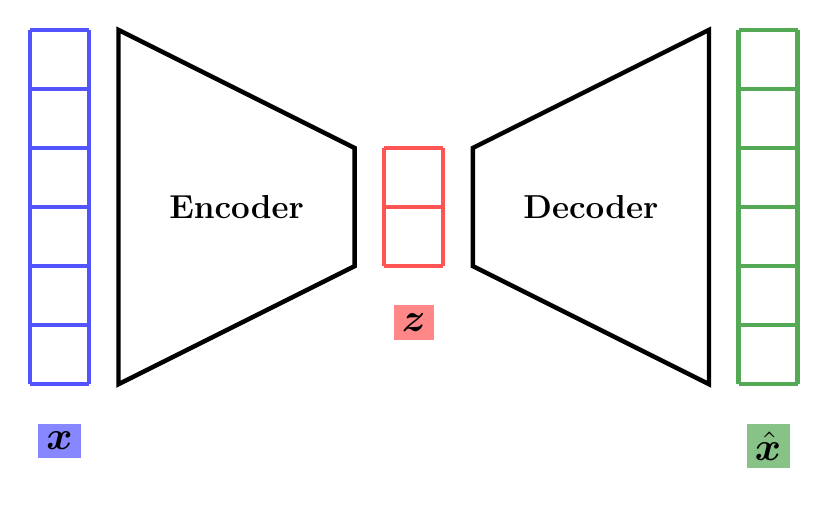
\begin{tikzpicture}[scale=0.75]
    % \draw[help lines, step=1] (-7, -4) grid (6, 4);

    \draw[step=1, ultra thick, draw=blue!67] (-7, -3) grid (-6, 3);

    \draw[step=1, ultra thick, draw=Green!67] (5, -3) grid (6, 3);

    \draw[step=1, ultra thick, draw=red!67] (-1, -1) grid (0, 1);

    \draw[ultra thick] (-5.5, -3) -- (-1.5, -1) -- (-1.5, 1) -- (-5.5, 3) -- cycle;

    \draw[ultra thick] (4.5, -3) -- (0.5, -1) -- (0.5, 1) -- (4.5, 3) -- cycle;

    \node[anchor=north] at (-6.5, -3.5) {\highlightdark{blue}{\Large $\bm{x}$}};
    \node[anchor=north] at (-0.5, -1.5) {\highlightdark{red}{\Large $\bm{z}$}};
    \node[anchor=north] at (5.5, -3.5) {\highlightdark{Green}{\Large $\hat{\bm{x}}$}};

    \node[] at (-3.5, 0) {\large \textbf{Encoder}};
    \node[] at (2.5, 0) {\large \textbf{Decoder}};

  \end{tikzpicture}

  \bigskip

  Many (linear) dimensionality reduction techniques in machine learning can actually be re-interpreted as variations around the theme of SVD.

  \vfill
\end{frame}






% \begin{frame}{N.\ Wiener's classification}
%   \centering
%   \vfill
%
%   \begin{tikzpicture}
%     %\draw[help lines, step=1] (-7, -3) grid (7, 3);
%
%     \draw[thick, white, fill=black] (-2, 0) circle (3);
%     \draw[thick, black,fill=white] (2, 0) circle (3);
%
%     \begin{scope}
%       \clip (-2, 0) circle (3);
%       \clip (2, 0) circle (3);
%       \fill[thick, black, fill=gray!40] (0, 0) circle (3);
%     \end{scope}
%
%     \node[anchor=east] at (-2, -3.5) {\textbf{Black box models}};
%     \node[anchor=west] at (2, -3.5) {\textbf{White box models}};
%
%     \node at (-2, 0) (A) {};
%     \path (A) ++(135:2.75) node[anchor=west] {Feedforward nets};
%     \path (A) ++(160:2.95) node[anchor=west] {Reinforcement};
%     \path (A) ++(170:2.8) node[anchor=west] {learning};
%     \path (A) ++(195:2.95) node[anchor=west] {Image classification};
%     \path (A) ++(220:2.95) node[anchor=west] {Model-free inference};
%
%
%     \node at (2, 0) (B) {};
%     \path (B) ++(45:2.75) node[anchor=east] {\textcolor{black}{First principles}};
%     \path (B) ++(20:2.75) node[anchor=east] {\textcolor{black}{Newton's eq.}};
%     \path (B) ++(0:2.9) node[anchor=east] {\textcolor{black}{Maxwell's eq.}};
%     \path (B) ++(-20:2.9) node[anchor=east] {\textcolor{black}{Differential eq.}};
%     \path (B) ++(-45:2.95) node[anchor=east] {\textcolor{black}{Parameter inference}};
%
%   \end{tikzpicture}
%
%   \vfill
% \end{frame}
%
% \begin{frame}{Example: Face recognition}
%   two faces with arrows
% \end{frame}
%
% \begin{frame}{Example: Face recognition}
%   overview figure of the SIAM paper
% \end{frame}
%
% \begin{frame}{Example: System identification}
%
% \end{frame}
%
% \section{A brief overview of SVD}
% \begin{frame}
%   \sectionpage
% \end{frame}
%
% \begin{frame}
%   \vfill
%
%
%   \begin{tcolorbox}[
%     enhanced,
%     coltitle=black,
%     coltext=white,
%     colback=black,
%     title=\textbf{Singular value decomposition},
%     frame style tile={width=\paperwidth}{background.jpg}
%     ]
%
%     \begin{overprint}
%
%       \onslide<1>
%       \large
%       \[
%       \bm{A} = \bm{U} \boldsymbol{\Sigma} \bm{V}^T
%       \]
%
%       \onslide<2>
%       \large
%       \[
%       \begin{bmatrix}
%         \bm{0} & \bm{A} \\
%         \bm{A}^T & \bm{0}
%       \end{bmatrix}
%       \begin{bmatrix}
%         \bm{u}_i \\ \bm{v}_i
%       \end{bmatrix}
%       =
%       \sigma_i
%       \begin{bmatrix}
%         \bm{u}_i \\ \bm{v}_i
%       \end{bmatrix}
%       \]
%
%     \end{overprint}
%   \end{tcolorbox}
%
%   \bigskip
%
%   Generalization of the \emph{eigenvalue decomposition} to \textbf{non-square matrices} by E. Beltrami (1873) and C. Jordan (1874).
%   The first efficient numerical algorithm was developed by G.\ Golub \emph{et al.} in the late 1960s.
%
%   \vfill
% \end{frame}
%
% \begin{frame}
%   Schematic SVD
% \end{frame}
%
% \begin{frame}{Geometric interpretation}
%
% \end{frame}
%
% \begin{frame}{Ordinary least-squares}
%   \vfill
%   \begin{minipage}{.48\textwidth}
%     \begin{overprint}
%       \onslide<1>
%       \Large
%       \[
%       \minimize_{\bm{x}} \dfrac{1}{2} \| \bm{Ax} - \bm{b} \|_2^2
%       \]
%
%       \onslide<2>
%       \Large
%       \[
%       \hat{\bm{x}} = \bm{A}^{\dagger} \bm{b}
%       \]
%
%       \onslide<3>
%       \Large
%       \[
%       \hat{\bm{x}} = \bm{V} \boldsymbol{\Sigma}^{-1} \bm{U}^T \bm{b}
%       \]
%     \end{overprint}
%   \end{minipage}%
%   \hfill
%   \begin{minipage}{.48\textwidth}
%     \large
%     \[
%     \begin{bmatrix}
%       ~ & ~ & ~ & ~ & ~ \\
%       ~ & ~ & ~ & ~ & ~ \\
%       ~ & ~ & ~ & ~ & ~ \\
%       ~ & ~ & ~ & ~ & ~ \\
%       ~ & ~ & \bm{A} & ~ & ~ \\
%       ~ & ~ & ~ & ~ & ~ \\
%       ~ & ~ & ~ & ~ & ~ \\
%       ~ & ~ & ~ & ~ & ~ \\
%       ~ & ~ & ~ & ~ & ~
%     \end{bmatrix}
%     \begin{bmatrix}
%       ~ \\ ~ \\ \bm{x} \\ ~ \\ ~
%     \end{bmatrix}
%     =
%     \begin{bmatrix}
%       ~ \\ ~ \\ ~ \\ ~ \\ \bm{b} \\ ~ \\ ~ \\ ~ \\ ~
%     \end{bmatrix}
%     \]
%   \end{minipage}
%   \vfill
% \end{frame}
%
% \begin{frame}{Low-rank approximation}
%   \vfill
%
%   \begin{minipage}{.48\textwidth}
%     \begin{overprint}
%       \onslide<1>
%       \Large
%       \[
%       \begin{aligned}
%         \minimize_{\hat{\bm{A}}} & \| \bm{A} - \hat{\bm{A}} \|_F^2 \\
%         \subto & \mathrm{rank~} \hat{\bm{A}} = r
%       \end{aligned}
%       \]
%
%       \onslide<2>
%       \Large
%       \[
%       \hat{\bm{A}} = \sum_{i=1}^k \sigma_i \bm{u}_i \bm{v}_i^T
%       \]
%     \end{overprint}
%   \end{minipage}%
%   \hfill
%   \begin{minipage}{.48\textwidth}
%   \end{minipage}
%
%   \vfill
% \end{frame}
%
% \begin{frame}{Orthogonal Procrustes problem}
%   \vfill
%   \begin{minipage}{.48\textwidth}
%     \begin{overprint}
%       \onslide<1>
%       \large
%       \[
%       \begin{aligned}
%         \minimize_{\bm{R}} & \| \bm{RA} - \bm{B} \|_F \\
%         \subto & \bm{R}^T \bm{R} = \bm{I}
%       \end{aligned}
%       \]
%
%       \onslide<2>
%       \large
%       \[
%       \bm{BA}^T = \bm{U} \boldsymbol{\Sigma} \bm{V}^T
%       \]
%
%       \onslide<3>
%       \large
%       \[
%       \bm{R} = \bm{UV}^T
%       \]
%
%     \end{overprint}
%   \end{minipage}%
%   \hfill
%   \begin{minipage}{.48\textwidth}
%     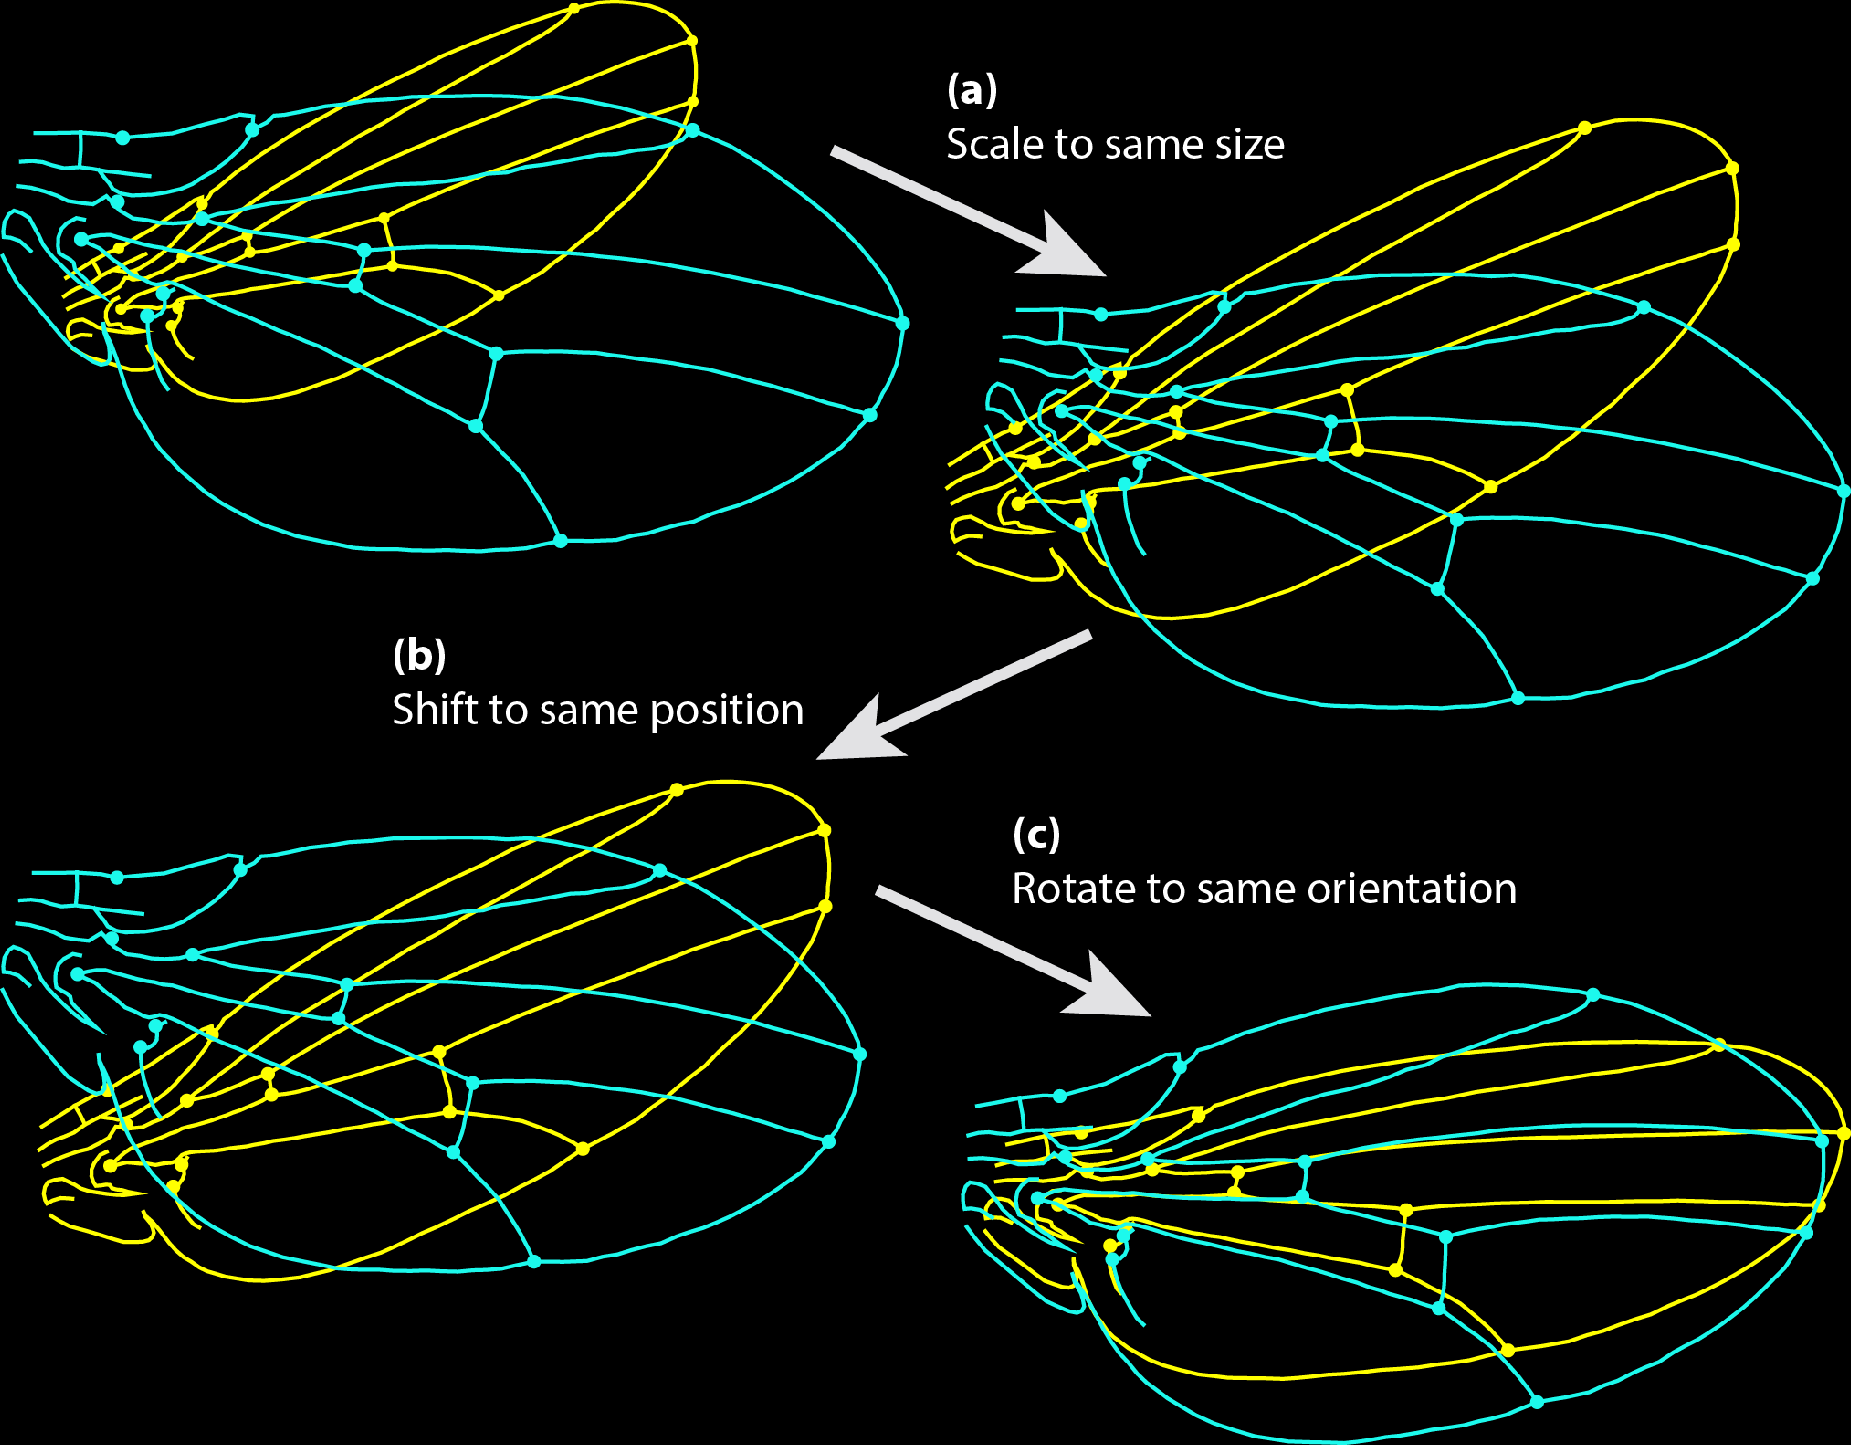
\includegraphics[width=\textwidth]{procrustes}
%   \end{minipage}
%   \vfill
% \end{frame}
%
% \section{SVD in data-driven modeling}
% \begin{frame}
%   \sectionpage
% \end{frame}
%
% \begin{frame}
%   \vfill
%
%   \Large
%
%   \[
%   \bm{y} = \bm{Kx} + \varepsilon
%   \]
%
%   \vfill
% \end{frame}
%
% \begin{frame}{Linear deconvolution problem}
%   Schematic of a linear system
% \end{frame}
%
% \begin{frame}{Linear deconvolution problem}
%   Schematic of deconvolution
% \end{frame}
%
% \begin{frame}
%   \vfill
%
%   \Large
%
%   \[
%   \bm{y} = \bm{Kx} + \varepsilon
%   \]
%
%   \vfill
% \end{frame}
%
% \begin{frame}
%
% \end{frame}
%
% \begin{frame}
%
%   \vfill
%
%   \begin{tcolorbox}[
%       enhanced,
%       coltitle=black,
%       coltext=white,
%       colback=black,
%       title=\textbf{Fundamental problem of component analysis},
%       frame style tile={width=\paperwidth}{background.jpg}
%     ]
%
%     \begin{overprint}
%       \onslide<1>
%       \large
%       \[
%       \begin{aligned}
%         \minimize_{\bm{K}} & \| \bm{M}^{\frac12} \left( \bm{Y} - \bm{KX} \right) \|_F \\
%         \subto & \mathrm{rank~} \bm{K} = r.
%       \end{aligned}
%       \]
%
%       \onslide<2>
%       \large
%       \[
%       \begin{aligned}
%         \minimize_{\bm{P}, \bm{Q}} & \| \bm{M}^{\frac12}  \left( \bm{Y} - \bm{PQ}^T \bm{X} \right) \|_F \\
%         \subto & \bm{P}^T \bm{MP} = \bm{I}_r \quad \left( \mathrm{ou~} \bm{Q}^T \bm{XX}^T \bm{Q} = \bm{I}_r \right).
%       \end{aligned}
%       \]
%
%     \end{overprint}
%
%   \end{tcolorbox}
%
%   \vfill
% \end{frame}
%
% \begin{frame}
%   \vfill
%
%   \Large
%   \[
%   \begin{bmatrix}
%     \bm{M} & \bm{0} \\
%     \bm{0} & \bm{0}
%   \end{bmatrix}
%   \begin{bmatrix}
%     \bm{p}_i \\ \bm{q}_i
%   \end{bmatrix}
%   \lambda_i
%   =
%   \begin{bmatrix}
%     \bm{0} & \bm{M} \bm{C}_{\bm{yx}} \\
%     \bm{C}_{\bm{xy}} \bm{M} & - \bm{C}_{\bm{xx}}
%   \end{bmatrix}
%   \begin{bmatrix}
%     \bm{p}_i \\ \bm{q}_i
%   \end{bmatrix}
%   \]
%
%   \vfill
% \end{frame}
%
% \begin{frame}{Proper Orthogonal Decomposition}
%   \vfill
%
%   \begin{minipage}{.38\textwidth}
%     \begin{tcolorbox}[
%         enhanced,
%         coltitle=black,
%         coltext=white,
%         colback=black,
%         title=\textbf{POD eigenproblem},
%         frame style tile={width=\paperwidth}{background.jpg}
%       ]
%       \large
%       \[
%       \bm{M} \bm{p}_i \lambda_i = \bm{C}_{\bm{xx}} \bm{p}_i
%       \]
%
%       \smallskip
%     \end{tcolorbox}
%   \end{minipage}%
%   \hfill
%   \begin{minipage}{.58\textwidth}
%     POD is recovered if $\bm{X} = \bm{Y}$ and $\bm{P} = \bm{Q}$.
%     It aims at characterizing the second order statistics of the random variable $\bm{x}$.
%   \end{minipage}
%
%   \vfill
% \end{frame}
%
% \begin{frame}
%   \vfill
%
%   \begin{minipage}{.48\textwidth}
%
%     \centering
%     \textbf{Complex Ginzburg-Landau equation}
%
%     \[
%     \dfrac{\partial q}{\partial t} = -U \dfrac{\partial q}{\partial x} + \mu(x) q + \gamma \dfrac{\partial^2 q}{\partial x^2} - \beta \vert q \vert^2 q
%     \]
%   \end{minipage}%
%   \hfill
%   \begin{minipage}{.48\textwidth}
%   \end{minipage}
%
%   \vfill
% \end{frame}
%
% \begin{frame}
%   \vfill
%
%   \begin{minipage}{.48\textwidth}
%     Covariance matrix
%   \end{minipage}%
%   \hfill
%   \begin{minipage}{.48\textwidth}
%     Eigenspectrum
%   \end{minipage}
%
%   \vfill
% \end{frame}
%
% \begin{frame}
%   \vfill
%
%   \begin{minipage}{.48\textwidth}
%     POD mode
%   \end{minipage}%
%   \hfill
%   \begin{minipage}{.48\textwidth}
%     Phase portrait
%   \end{minipage}
%
%   \vfill
% \end{frame}
%
% \begin{frame}{Galerkin projection}
%
% \end{frame}

\end{document}
